\documentclass[11pt]{article}
\usepackage[T1]{fontenc}
\usepackage{calc}
\usepackage{setspace}
\usepackage{multicol}
\usepackage{fancyheadings}
\usepackage{grffile}
\usepackage[round]{natbib}
\usepackage{subcaption}

\usepackage{siunitx}
\sisetup{input-symbols=(), group-digits  = false}
 
\usepackage{graphicx}
\usepackage{color}
\usepackage{rotating}
%\usepackage{harvard}
%\usepackage{aer}
%\usepackage{aertt}
\usepackage{verbatim}
\usepackage{array}
\usepackage{multirow}

\setlength{\voffset}{-0.25in}
\setlength{\topmargin}{0pt}
\setlength{\hoffset}{-0.25in}
\setlength{\oddsidemargin}{0pt}
\setlength{\headheight}{0pt}
\setlength{\headsep}{0in}
\setlength{\marginparsep}{0pt}
\setlength{\marginparwidth}{0pt}
\setlength{\marginparpush}{0pt}
\setlength{\footskip}{.2in}
\setlength{\textwidth}{7in}
\setlength{\textheight}{9.4in}
\setlength{\parskip}{0pc}

\renewcommand{\baselinestretch}{1.7}

\newcommand{\bi}{\begin{itemize}}
\newcommand{\ei}{\end{itemize}}
\newcommand{\be}{\begin{enumerate}}
\newcommand{\ee}{\end{enumerate}}
\newcommand{\bd}{\begin{description}}
\newcommand{\ed}{\end{description}}
\newcommand{\prbf}[1]{\textbf{#1}}
\newcommand{\prit}[1]{\textit{#1}}
\newcommand{\beq}{\begin{equation}}
\newcommand{\eeq}{\end{equation}}
\newcommand{\bdm}{\begin{displaymath}}
\newcommand{\edm}{\end{displaymath}}
\newcommand{\script}[1]{\begin{cal}#1\end{cal}}
%\newcommand{\citee}[1]{\citename{#1} (\citeyear{#1})}
\newcommand{\citee}[1]{\citet{#1}}
%\newcommand{\citee}[1]{\citeauthor{#1} (\citeyear{#1})}
\newcommand{\h}[1]{\hat{#1}}
\newcommand{\ds}{\displaystyle}
\newcommand{\normal}{\mathcal{N}}
\newcommand{\app}
{
\appendix
}

%\newcommand{\appsection}[1]
%{
%\let\oldthesection\thesection
%\renewcommand{\thesection}{Appendix \oldthesection}
%\section{#1}\let\thesection\oldthesection
%\renewcommand{\theequation}{\thesection\arabic{equation}}
%\setcounter{equation}{0}
%}

\newcommand{\appsection}[1]
{
\section{#1}
\renewcommand{\theequation}{\thesection\arabic{equation}}
\setcounter{equation}{0}
}


%\pagestyle{empty}
%\pagestyle{fancyplain}
%\lhead{}
%\chead{Fiscal Policy Uncertainty and Its Macroeconomic Consequences}
%\rhead{\thepage}
%\lfoot{}
%\cfoot{}
%\rfoot{}
\pagestyle{plain}

\begin{document}

\begin{titlepage}
\begin{singlespace}
\title{Fiscal Policy Uncertainty and Its Macroeconomic Consequences}
\date{\today}
\author{
James Murray\footnote{\textit{Mailing address}: 1725 State St., La Crosse, WI  54601. \textit{Phone}: (608)406-4068.\newline  \textit{E-mail}: jmurray@uwlax.edu.}\\Department of Economics\\University of Wisconsin - La Crosse
}

\maketitle

\thispagestyle{empty}

\abstract{I examine fiscal policy uncertainty in a context where market participants learn about the conduct of fiscal policy with regression rules for dependent variables including tax revenue, net transfers, government spending, and government debt.  The explanatory variables include lagged fiscal policy, lagged government debt, and macroeconomic outcomes including real GDP, consumption, investment, and the unemployment rate.  They re-run these regressions each quarter as a new observation becomes available, updating their understanding of the conduct of fiscal policy.  I use the root mean squared errors as measures for fiscal policy uncertainty.  I use autoregressive distributed lag (ARDL) models to estimate the effect fiscal uncertainty has on macroeconomic outcomes including real GDP, consumption, investment and unemployment.  I find that the common component for fiscal policy uncertainty has adverse effects on real GDP, consumption, and investment.  I find the buildup of fiscal policy uncertainty from 2005 through 2009 leads to a decline in real GDP growth by about 2 percentage points.  I demonstrate that these finding are robust to lag specifications for the ARDL models and parameter specifications for the learning process.}\\

\noindent \textit{Keywords}: Fiscal policy, uncertainty, adaptive expectations, learning, autoregressive distributed lag models. \\
\noindent \textit{JEL classification}: E32, E62.
\end{singlespace}
\end{titlepage}

\newpage

\section{Introduction}

In recent years, the United States experienced a severe financial crisis, the worst economic downturn since the Great Depression, and unprecedented fiscal and monetary policy actions have been accompanied with only a slow recovery.  Add to this strong political partisan divisions, with some arguing for more economic stimulus or more economic assistance for those in need, and others arguing for contraction in government spending and transfers. 

These economic and political hardships have come with renewed interest in what effect uncertainty concerning government policy has on the macroeconomy.  In a July 2012 monetary policy report to the U.S. Congress, then Federal Reserve chairman Ben Bernanke suggested that the most effective way that Congress can support the economic recovery is to design long-run policy that removes uncertainty concerning the fiscal stance of the Federal Government, which he suggested could help boost consumer and business confidence.\footnote{See \citee{bernanke2012}.  In closing his discussion of risks to the U.S. economic outlook, Bernanke's precise words were, ``The most effective way that the Congress could help to support the economy right now would be to work to address the nation's fiscal challenges in a way that takes into account both the need for long-run sustainability and the fragility of the recovery. Doing so earlier rather than later would help reduce uncertainty and boost household and business confidence.''}  

The purpose of this paper is to introduce a new way to quantify fiscal policy uncertainty that is based on a realistic framework for forming expectations, and use this measure to estimate the effect that fiscal policy uncertainty has the macroeconomy.  I construct a measure for fiscal policy uncertainty using least-squares learning, an expectations mechanism where market participants have a more restricted information set than what is typically assumed in rational expectations models.  It is common when using rational expectations to assume that market participants have knowledge of the equations and parameters governing fiscal policy behavior, and the only source of uncertainty is in future realizations of a stochastic shock (though I cite some notable exceptions concerning fiscal policy in the next section).  \citee{eh2011} argue that rational expectations models like these violate the cognitive consistency principle.  That is, the rational expectations framework assumes that market participants have a higher degree of knowledge concerning the law of motion for economic variables than the economists themselves who write down the model.  

I suppose that market participants' knowledge and expectations behavior is similar to what might be expected of an applied econometrician.  Market participants have statistical models for the behavior for fiscal policy variables, and they estimate these models in each period with data that precedes it.  Expectations evolve according to least-squares learning in the style of \citee{eh2001}.  In each new period, a new observation becomes available and market participants re-estimate their regressions and the prediction from the updated regression serves as their expectation.  Following the method in \citee{herromurray} in their examination of monetary policy uncertainty, I interpret the root mean squared errors from these regressions as fiscal policy uncertainty, as it is a measure of fiscal policy variability that is not explained by past behavior or previous data.  Also, the variance for forecasts for fiscal policy based on these regression models are direct functions of the mean squared error.  \citee{orlik2013} have a similar construction for general economic uncertainty in an environment which also includes model uncertainty.  

I obtain measures of fiscal policy uncertainty for government expenditures, tax revenue, net transfers and government debt.  These measures are all highly correlated, so I estimate and isolate the common component using a standard dynamic factor model.  To determine the effect fiscal policy uncertainty has on the macroeconomy, I estimate autoregressive distributed lag (ARDL) models for dependent variables including real GDP, consumption, investment, and unemployment.  The set of explanatory variables in each ARDL includes lags of a larger set of macroeconomic variables, lagged fiscal policy variables, and fiscal policy uncertainty variables, including separate measures for each of the four fiscal policy variables mentioned above and the common component for fiscal policy uncertainty.  To check for robustness, I run a number of specifications with different lag lengths and different specifications for market participants' regression equations.  I find consistent evidence that government expenditures uncertainty and tax uncertainty negatively affect investment, while transfers uncertainty is related to a decrease in unemployment.  While less robust to the model specification, I also find evidence that tax uncertainty and government debt uncertainty negatively affects consumption and real GDP.  The common component of fiscal policy uncertainty is shown to be contractionary in nearly all specifications.

\section{Literature}

\citee{fvetal2011}, \citee{born2011}, and \citee{johannsen2012} find significant evidence of time-varying volatility in fiscal shocks.  These papers focus on uncertainty specifically regarding fiscal policy and they complement a larger literature that examines the effect of time-varying economic uncertainty on business cycles (see, for example, \citee{justprim2008}, \citee{bloom2009}, \citee{fvetal2011aer}, and \citee{bloom_uncertainbus}).  Using a New Keynesian business cycle model calibrated to the U.S. economy, \citee{fvetal2011} find that fiscal uncertainty has stagflationary effects.  An increase in the volatility of fiscal shocks leads to a decrease economic activity for several quarters and an increase in aggregate price level through the optimal price setting channel with sticky prices.  \citee{born2011} estimate a similar model with U.S. data and find that fiscal uncertainty is unlikely to be a driving factor explaining U.S. business cycles.  They demonstrate that there are counteracting partial equilibrium effects that can mute the effects of uncertainty.  \citee{fvetal2011} defend the concern to place on fiscal policy uncertainty, but not because typical fiscal volatility shocks should be on average an important driver of business cycles.  Rather, the occasional large shock has large adverse effects.  This should especially be of concern when an increase in policy risk comes at the same time that policy is attempting to counteract economic contraction, which is arguably the case in the wake of the Great Recession in the United States.\footnote{\citee{fvetal2011} and \citee{born2011} do not explicitly model such a case.  Fiscal uncertainty shocks are modeled as independent innovations to an autoregressive conditional heteroskedastic process.}  

Some studies do suggest that fiscal policy uncertainty may have been a particularly important concern during the Great Recession and subsequent recovery.  \citee{johannsen2012} demonstrates that the effect of fiscal policy uncertainty is magnified when monetary policy is at its zero lower bound.  \citee{baker2013} construct their own measure of economic policy uncertainty based on the frequency of newspaper headlines concerning policy uncertainty in ten leading news papers, the number of federal tax code provisions that are soon due to expire, and the extent of disagreement among professional forecasters.  They find that an increase in policy uncertainty in the magnitude that they find from 2006-2011 reduces industrial production by 2.5\% and total employment by 2.3 million.

A related literature on fiscal policy uncertainty focuses specifically on uncertainty concerning long-term fiscal financing.  \citee{leeper_ej} show that when there is uncertainty considering the timing and composition (whether spending-based or tax-based) of fiscal consolidations, economic agents do not rule out the possibility for undesirable conditions for an upcoming fiscal consolidation (for example, a tax-based consolidation).  Expectations and behavior react immediately which can have contractionary effects (relative to a situation where a more desirable composition for fiscal contraction was known with certainty).  \citee{davig_leeper_walker} show that uncertainty regarding the government's long-term plan for financing entitlement programs can be stagflationary.  When the costs for entitlement programs follow unsustainable paths, it is expected that either the government will eventually renege on its obligations or that the monetary authority will switch to a passive policy that does not react more than one-to-one to inflation, allowing surprise increases in the price level that decrease the real value of government debt and transfer obligations.  When agents put a positive probability on the latter, it can create an environment of suppressed economic activity and inflation that even an active monetary authority can adequately control.

\citee{richter2013} and \citee{davig2013} consider models and expectations environments where there is uncertainty on upcoming policy changes.  \citee{davig2013} construct a model of expiring tax provisions in which uncertainty exists whether a tax policy will expire at a predetermined expiration date, or if it will be extended.  They show that this uncertainty can lead to a drop in investment and unemployment.  Motivated by situations like expiring tax policies and uncertain possibility for extension, \citee{richter2013} develop a model with regime switching in the long-run debt to GDP level.  They show that uncertainty may be welfare improving or welfare reducing, depending on whether agents' expectations are consistent with future realizations for the debt to GDP state.  They suggest that the recent U.S. experience concerning the expiring Bush-era tax cuts was likely contractionary.  When economic agents underestimated the debt target, and therefore overestimated the future flow of taxes, they under-invested relative to what they would do under certainty.  

The expectations framework to model how agents perceive fiscal policy in the present paper is most similar to \citee{hollmatt}.\footnote{\citee{hollmatt} supposes agents use Bayesian learning to update their beliefs on the behavior of fiscal policy whereas the present paper uses recursive least-squares learning.}  These authors also suppose that agents do not know the coefficients governing a fiscal policy rule, and they update their estimates recursively based on the relationship between past fiscal policy and past macroeconomic outcomes.  They find that if the government permanently increases spending and if agents are left to learn about the change in behavior, this leads to a significant prolonged decrease in real GDP relative to the case with full information on the fiscal policy change.  Furthermore, they find that short-run learning dynamics concerning the change in fiscal policy leads to more short-run macroeconomic volatility.

\section{Expectations}

\subsection{Least Squares Learning}
Market participants expect that fiscal policy variables follow feedback rules that respond to economic conditions, past behavior of fiscal policy, and the recent level of government debt.  Let $f_t = [g_t~ r_t~ n_t~ b_t]'$ denote the time $t$ vector of fiscal policy variables under consideration, where $g_t$ is real government expenditures, $r_t$ is real tax revenue, $n_t$ is real net transfers, and $b_t$ is real government debt.  All of these variables are observed at the quarterly frequency, quantities are measured in per-capita terms and taken as a ratio of the previous quarter's level of real GDP per capita, and all fiscal variables are an aggregate of U.S. federal, state, and local governments.  Market participants estimate the following regression every period to update their understanding of the conduct of fiscal policy:
\beq \label{eq:fiscalrule} f^{i}_{t} = \alpha^i_{0} + (\alpha^{i}_{f})' f_{t-1} + \alpha^i_{y} y_t + \alpha^i_c c_t + \alpha^i_I I_t + \alpha^i_u u_t + \epsilon^i_{t}, \eeq
Equation (\ref{eq:fiscalrule}) is estimated for each $f_{i,t}$, the $i$th fiscal policy variable in the vector, $f_t$.  The explanatory variables include real GDP ($y_t$), real consumption expenditures ($c_t$), real investment $I_t$, and unemployment ($u_t$).  Again, these variables are observed at a quarterly frequency, the quantities for real GDP, real consumption, and real investment are put in per-capita terms and expressed as a ratio of the previous quarter's level of real GDP per capita; and unemployment is expressed as a percentage rate.  

Equation (\ref{eq:fiscalrule}) is rich in its set of explanatory variables, but it includes important features from other fiscal feedback rules used in the macroeconomics literature.  In the most simple fiscal policy frameworks, such as in \citee{SchmittGrohe2007} and \cite{ChungDavigLeeper2007}, tax revenues only respond to past government debt-to-GDP.  \citee{DavigLeeper2006} also let tax revenues respond contemporaneously to government spending and the output gap, the latter which can be considered a combination of automatic stabilizers and discretionary policy to target real GDP.  \citee{Favero2003} use feedback rules on fiscal deficits, where deficits can exhibit persistence, and respond to debt-to-GDP, the output gap, and the interest rate net of the output growth rate.  

Equation (\ref{eq:fiscalrule}) contains many of these features.  By allowing each fiscal policy variable to respond to the vector, $f_{t-1}$, each fiscal policy variable can have persistence, and recent fiscal policy behavior may effect all the other fiscal policy variables.  The rule allows for all fiscal variables to respond to lagged debt-to-GDP as this is also included in $f_{t-1}$.  The feedback on output, consumption, investment, and unemployment allow for a rich set of discretionary policy and automatic stabilizers.

Market participants update their understanding of fiscal policy in each time period by re-estimating equation (\ref{eq:fiscalrule}) for each fiscal policy variable, using data up through period $t-1$.  Let $x_{t} = [1~ f'_{t-1}~ y_t~ c_t~ I_t~ u_t]'$ denote the vector of explanatory variables used to predict $f^i_{t}$, and let $\hat{\alpha}^{i,OLS}_{t}$ denote the associated vector of ordinary least-squares estimates for the coefficients.  The coefficient estimates for the $i$th fiscal policy variable are given by,
\beq \hat{\alpha}^{i,OLS}_{t} = \left( \frac{1}{t} \sum_{\tau=1}^{t} x_{t-\tau} x_{t-\tau}' \right)^{-1}  \left( \frac{1}{t} \sum_{\tau=1}^{t} x_{t-\tau}  f^i_{t-\tau} \right). \eeq
This can be re-written in the recursive form,
\beq \label{eq:olsln} \hat{\alpha}^{i,OLS}_t = \hat{\alpha}^{i,OLS}_{t-1} + \gamma_t  R_t^{-1} x_{t-1} \left(f^i_{t-1} - x_{t-1}'\hat{\alpha}^{i,OLS}_{t-1}\right) \eeq
\beq \label{eq:olslnR} R_t = R_{t-1} + \gamma_t \left(x_{t-1} x_{t-1}' - R_{t-1}\right), \eeq
where $\gamma_{t} = 1/t$ is the learning gain and is equal to the weight given to the most recent observation.  The recursive form illustrates the manner in which expectations formed by least-squares predictions are adaptive.  Equation (\ref{eq:olsln}) shows that the most recent estimate for the coefficient vector is equal to the previous estimate, plus a correction factor which depends on the weight given to the most recent observation ($\gamma_t$) and the size of the prediction error implied from the previous estimate (the term in parentheses on the right-hand-side).  

Absent of any stochastic shocks or changes in the structure of the data generating process, under ordinary least-squares the learning gain converges to zero, the coefficients converge to some set of values, and any dynamics or uncertainty due to adaptive expectations disappears.  If the learning gain were to be replaced with a constant, $\gamma_t=\gamma,~ \forall_t$, where $\gamma \in (0,1)$, adaptive expectations dynamics never disappears.  Repeated substitution of equation (\ref{eq:olsln}) with a constant learning gain leads to the weighted least squares estimate for the coefficients,
\beq \hat{\alpha}^{i}_{t} = \left( (1-\gamma) \sum_{\tau=1}^{t} \gamma^\tau x_{t-\tau} x_{t-\tau}' \right)^{-1}  \left( (1-\gamma) \sum_{\tau=1}^{t} \gamma^\tau x_{t-\tau}  f^i_{t-\tau} \right), \eeq
where $(1-\gamma) \gamma^\tau$ is the weight given to an observation from $\tau$ periods in the past.  Since the learning gain is less than one, weights decline geometrically with the age of the observation.  Common estimates for the learning gain for quarterly observations are around $0.01-0.02$ (see, for example, \citee{milani2007} or \citee{slobodyan_wouters_2012}).  This is roughly consistent with agents estimating regressions using a rolling window of between 50-100 observations, or about 12.5-25 years of quarterly data.

Constant-gain learning is useful when market participants suspect that structural changes are possible, but they are not endowed with a menu and probability set of possible structural changes.  Rather, agents put more weight on more recent observations that are more likely to represent the current data generating process.  This is likely the case with fiscal policy.  Structural changes can come from shifts in political power, shifts in the political value placed fiscal stimulus versus austerity, shifts in emphasis on using government spending versus taxes versus transfers, and changes in tax laws, spending programs, or transfer programs.

Because the learning process is nonlinear, it introduces a source of time-varying volatility in expectations and uncertainty, even in an otherwise linear model with constant-variance innovations.  The purpose of this paper is to quantify the size and evolution of uncertainty implied by least-squares learning, and measure the impact uncertainty concerning fiscal policy has on the macroeconomy.  
 
\subsection{Learning with Instrumental Variables}
The set of explanatory variables in agents' regressions includes concurrent values for output, consumption, investment, and unemployment, all of which are likely endogenous.  Following \citee{herromurray}, I present here a modified learning algorithm that allows market participants to account for endogeneity using instrumental variables (IV) and two-stage least squares (2SLS).  Let $w_t$ be the subset of variables in $x_t$ that are possibly endogenous, and $v_t$ be the remaining exogenous variables so that $x_t = [v_t'~ w_t']'$.  The exogenous variables include the lagged fiscal policy variables and the constant term.  All the other explanatory variables are concurrent macroeconomic variables and so they are possibly endogenous.  Let $z_t$ denote a vector that includes instruments and exogenous variables.  I suppose market participants use as instruments two lags each of all the endogenous variables and an additional two lags of each of the fiscal policy variables (the first lag is already an explanatory variable).

In the first stage, market participants estimate the following relationship to determine how much the endogenous variables can be explained only by instruments and exogenous variables,
\beq w^j_{t} = z_t ' \beta^j + \xi^j_{t}, \eeq
where superscript $j$ denotes the $j$th endogenous variable in vector $w_t$.  The weighted least-squares estimate for the first-stage coefficients is given by,
\beq \label{eq:iv1} \hat{\beta}^j_t = \left( (1-\gamma)  \sum_{\tau=1}^{t} \gamma^{\tau} z_{t-\tau} z_{t-\tau}' \right)^{-1}  \left( (1-\gamma)  \sum_{\tau=1}^{t} \gamma^{\tau} z_{t-\tau}  w^j_{t-\tau} \right), \eeq
and the predicted value for the endogenous vector is given by $\hat{w}^j_{t} = z_{t}' \hat{\beta}^j_t.$

Let $\hat{x}_t = [v_t'~ \hat{w}_{t}']'$ denote the explanatory variables used in the second stage regression, where endogenous variables in $x_{t}$ have been replaced with their predicted values from the first stage regression.  The IV estimates for the coefficients in the fiscal policy feedback rules are given by,
\beq \label{eq:iv2} \hat{\alpha}_t^{i,IV} = \left( (1-\gamma)  \sum_{\tau=1}^{t} \gamma^{\tau} \hat{x}_{t-\tau} \hat{x}_{t-\tau}' \right)^{-1}  \left( (1-\gamma)  \sum_{\tau=1}^{t} \gamma^{\tau} \hat{x}_{t-\tau}  f^i_{t-\tau} \right), \eeq
where again the $i$ superscript denotes the $i$th fiscal policy variable in vector $f_t$.  The 2SLS procedure can be written in the following recursive form,
\beq \label{lniv} \begin{array}{c}
\mbox{Stage 1:} \\ [0.5pc]
 \hat{\beta}^j_t = \hat{\beta}^j_{t-1} + \gamma \left(R_t^{S1}\right)^{-1} z_{t-1} \left(w^j_{t-1} - z_{t-1}'\hat{\beta}^j_{t-1}\right) \\ [0.5pc]
 R_t^{S1} = R_{t-1}^{S1} + \gamma \left(z_{t-1} z_{t-1}' - R_{t-1}^{S1}\right) \\ [0.5pc]
 \hat{w}^j_{t} = z_{t}' \hat{\beta}^j_t,~~~  \hat{x}_t = [v_t'~ \hat{w}_t']' \\ [1pc]
\mbox{Stage 2:} \\ [0.5pc]
 \hat{\alpha}_t^{i,IV} = \hat{\alpha}_{t-1}^{i,IV} + \gamma \left(R_t^{S2}\right)^{-1} \hat{x}_{t-1} \left(f^i_{t-1} - \hat{x}_{t-1}'\hat{\alpha}^i_{t-1}\right) \\ [0.5pc]
 R_t^{S2} = R_{t-1}^{S2} + \gamma \left(\hat{x}_{t-1} \hat{x}_{t-1}' - R_{t-1}^{S2}\right). 
\end{array} \eeq

The learning process requires initial conditions for coefficient vectors $\hat{\beta}^j_t$ and $\hat{\alpha}_t^{i,IV}$ and cross-product matrices $R_t^{S1}$ and $R_t^{S2}$.  To initialize these, I use a pre-sample of six years of quarterly data immediately preceding the sample period and estimate the 2SLS regression with a-priori equal weights on the observations.  

\subsection{Expectations and Uncertainty}
At each period in time, market participants acquire a new observation from the previous time period, re-estimate their regressions through period $t-1$ using the 2SLS procedure above, and finally evaluate how well they understand the conduct of fiscal policy by comparing actual fiscal policy with the predicted values implied by their regressions.  Market participants' time $t$ expectation for fiscal policy at time $t$ is given by,
\beq \label{eq:fpupred} \hat{f}^i_t = x_t' \hat{\alpha}_t^{i,IV}. \eeq
Notice that this predicted value is not a forecast from the previous time period, but an expectation for concurrent fiscal policy informed by concurrent macroeconomic conditions (given in $x_t$) and past fiscal policy behavior (given in $\hat{\alpha}_t^{i,IV}$).  The unexpected component of fiscal policy is given by,
\beq \hat{\epsilon}^i_t = f^i_t - \hat{f}^i_t = f^i_t - x_t' \hat{\alpha}_t^{i,IV}, \eeq
which is fiscal policy that is not explained by current economic conditions nor past fiscal policy behavior.  I measure fiscal policy uncertainty using a root mean squared aggregate of these residuals.   Specifically, I use a weighted root mean squared residual consistent with the constant-gain learning algorithm presented above, which is given by,
\beq \label{eq:fpu} m_{t}^i = \sqrt{ (1-\gamma) \ds \sum_{\tau=1}^{t} \gamma^{\tau} (f^i_{t-\tau} - x_{t-\tau}'\hat{\alpha}_{t-\tau}^{i,IV} )^2}. \eeq  
Because there is a regression model for each fiscal policy variable, $i$, including government spending, taxes, transfers, and government debt, the procedure allows one to quantify uncertainty regarding each type of fiscal policy.  Finally, this measure of fiscal policy uncertainty is solely a measure of uncertainty regarding fiscal policy, and does not conflate unexpected fiscal actions with unexpected macroeconomic outcomes, because concurrent macroeconomic outcomes are taken into account to form the expectation for the fiscal variables in equation (\ref{eq:fpupred}).
 
\subsection{Data}
The sample period spans 1960:Q3 to 2013:Q2 using U.S. quarterly data.  To set initial conditions for the learning process, I use a pre-sample period from 1954:Q3 through 1960:Q2.  The macroeconomic variables include real GDP, real consumption expenditures, real private domestic investment, and the civilian unemployment rate.  Real GDP, consumption, and investment come from the Bureau of Economic Analysis and are put in per-capita terms, and expressed as a ratio of real GDP per capita from the previous quarter.  The civilian unemployment rate is from the Bureau of Labor Statistics and expressed as a percentage.  The fiscal variables include government expenditures, tax revenue, net transfers, and government debt.  The first three come from the Bureau of Economic Analysis and government debt comes from the Federal Reserve Board of Governors Financial Accounts of the United States.  The fiscal variables are also in real per-capita terms and expressed as a ratio of the GDP per capita from the previous quarter.  Government expenditures is government consumption plus government investment, and includes federal, state, and local governments.  Tax revenue is government current tax receipts, which includes all levels of government and is put in real terms using the GDP Implicit Price Deflator.  Transfers are government current transfer payments, specifically government social benefits, and is also put into real terms using the GDP deflator.  Government debt is defined as the sum of federal government debt securities and state and local government credit market instruments, excluding employee retirement funds.  Government debt is put into real terms using the GDP deflator.

\subsection{Expectations and Uncertainty}\label{s:exp}

\begin{figure}\caption{Least-Squares Learning Predictions}\label{fg:forecasts0.02}
\begin{center}
\begin{tabular}{cc}
\multicolumn{2}{c}{Learning Gain = 0.02} \\ [0.5pc]
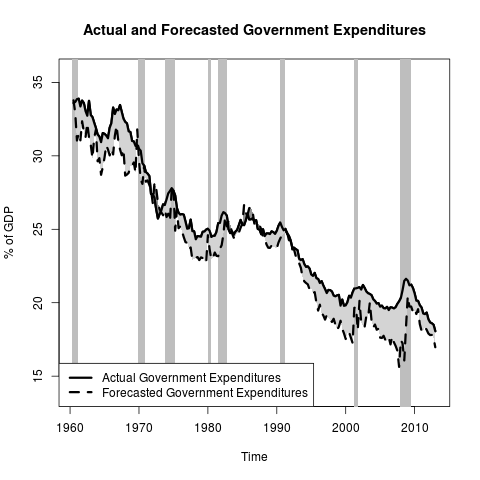
\includegraphics[scale=0.45]{./results/pics0.02/pred_gov.png} & 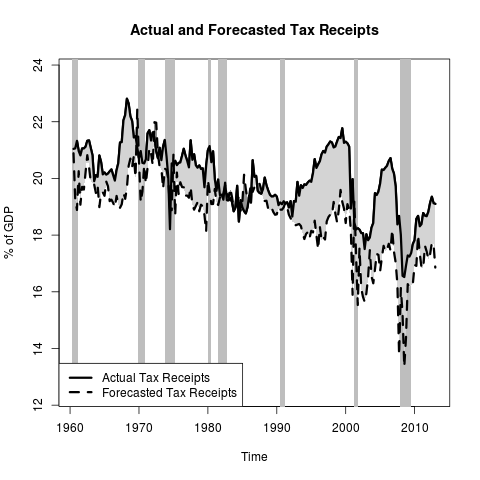
\includegraphics[scale=0.45]{./results/pics0.02/pred_tax.png} \\
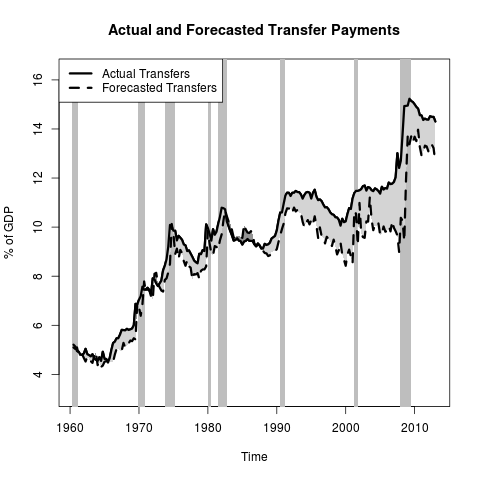
\includegraphics[scale=0.45]{./results/pics0.02/pred_transfers.png} & 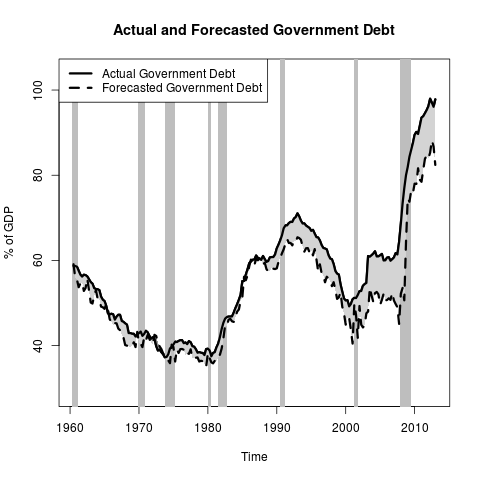
\includegraphics[scale=0.45]{./results/pics0.02/pred_debt.png}  
\end{tabular}
\end{center}
\end{figure} 

\begin{figure}\caption{Least-Squares Learning Prediction Errors}\label{fg:fe0.02}
\begin{center}
\begin{tabular}{cc}
\multicolumn{2}{c}{Learning Gain = 0.02} \\ [0.5pc]
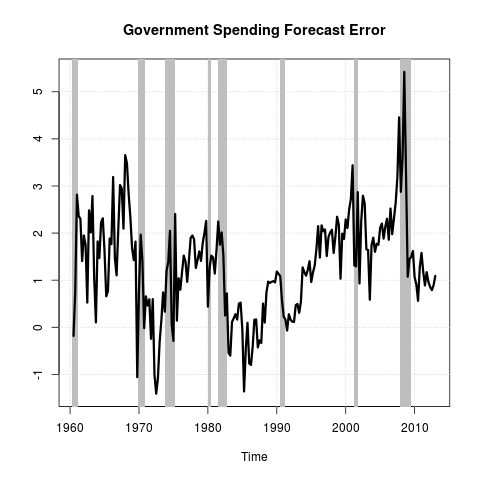
\includegraphics[scale=0.45]{./results/pics0.02/fe_gov.png} & 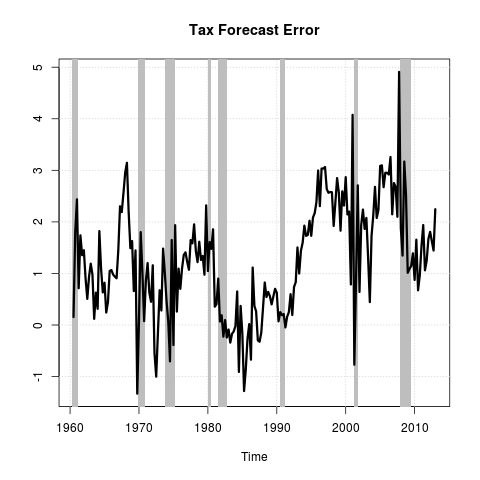
\includegraphics[scale=0.45]{./results/pics0.02/fe_tax.png} \\
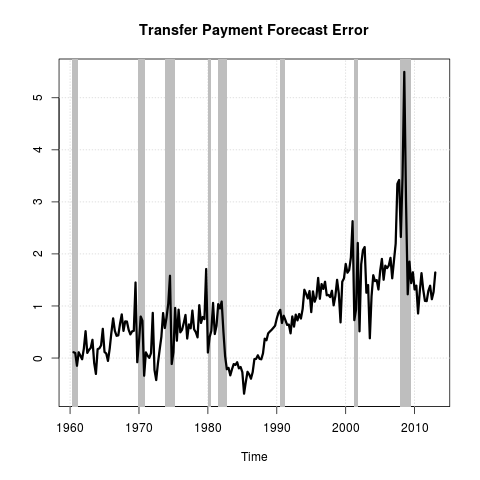
\includegraphics[scale=0.45]{./results/pics0.02/fe_transfers.png} & 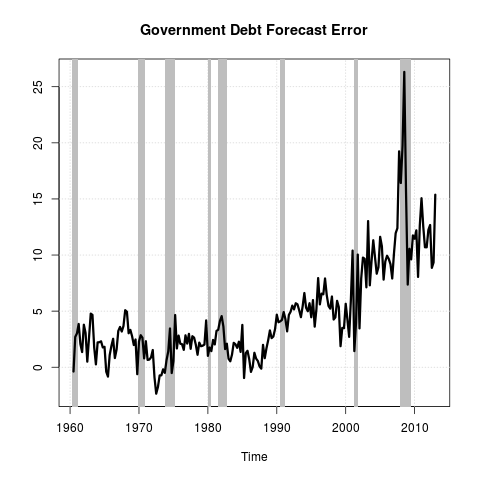
\includegraphics[scale=0.45]{./results/pics0.02/fe_debt.png}  
\end{tabular}
\end{center}
\end{figure} 

Figure \ref{fg:forecasts0.02} shows plots of the actual fiscal policy variables (solid line) and the associated least-squares expectations (dashed line) for each fiscal policy variable with a learning gain equal to 0.02.  Constant gain least-squares leads to underestimates for all of the fiscal policy variables over most of the sample.  Figure \ref{fg:fe0.02} shows plots of the prediction error.  For government spending and tax revenues, constant gain least-squares underestimates actual fiscal policy by about 1\% to 2\% of real GDP over much of the sample period, with larger prediction errors occurring after 1990.  Transfers are underestimated by about 0\% to 1\% of real GDP in the first 30 years of the sample, and between 1\% and 2\% of real GDP since 1990, with spikes of 2.5\% and over 5\% of real GDP occurring in 2001 and 2008.  Government debt is underestimated by about 0\% to 5\% of real GDP from 1960-1990, then the prediction error grows to between 5\% and 15\% of real GDP afterwards.  There is another seemingly permanent climb in the average prediction error for government debt in 2000.  There is a large spike in all of the estimated residuals at the onset of the great recession in 2008.  Note that since the least-squares learning regression models condition on concurrent macroeconomic variables, the residuals reflect unexpected fiscal responses, and not unexpected macroeconomic conditions.

\begin{figure}\caption{Fiscal Policy Uncertainty}\label{fg:fpu0.02}
\begin{center}
\begin{tabular}{cc}
\multicolumn{2}{c}{Learning Gain = 0.02} \\ [0.5pc]
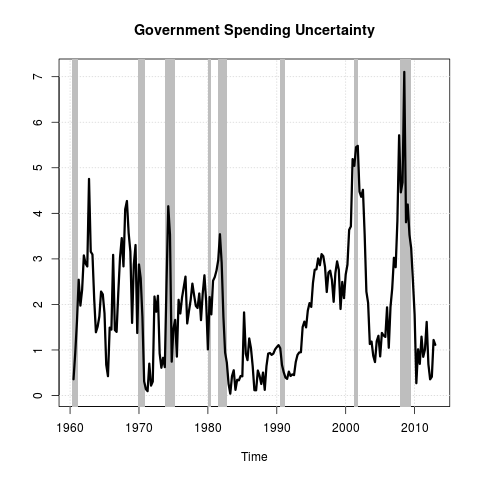
\includegraphics[scale=0.45]{./results/pics0.02/fpu_gov.png} & 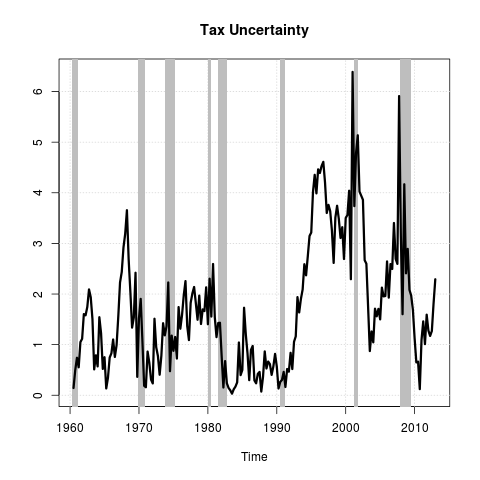
\includegraphics[scale=0.45]{./results/pics0.02/fpu_tax.png} \\
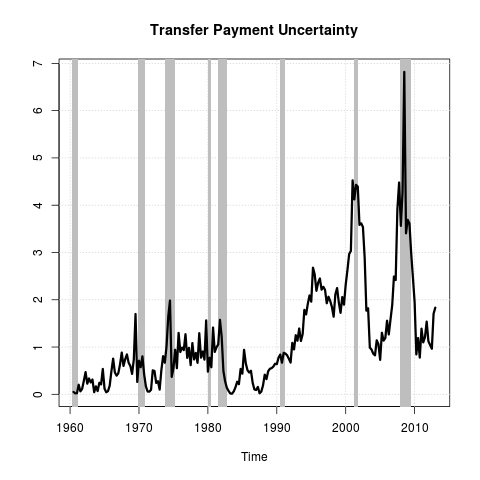
\includegraphics[scale=0.45]{./results/pics0.02/fpu_transfers.png} & 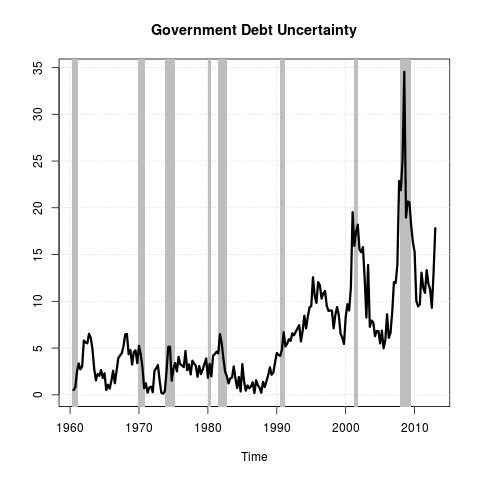
\includegraphics[scale=0.45]{./results/pics0.02/fpu_debt.png}  
\end{tabular}
\end{center}
\end{figure} 

Figure \ref{fg:fpu0.02} shows plots of fiscal policy uncertainty.  The figure shows that the buildups of prediction errors associated with the economic expansion from 1991 through 2001 led to a steady increase in fiscal policy uncertainty leading up to the 2001 recession.  Fiscal policy uncertainty comes down quickly following the recession, but climbs during the years prior to the great recession, reaching record or near-record levels at the onset of the recession.  The record levels of fiscal policy uncertainty during the great recession reach near 7\% of real GDP for government expenditures, near 6\% of real GDP for tax revenue, near 7\% of real GDP for transfers, and nearly 35\% of real GDP for government debt.  

The evolution for expectations and uncertainty with alternative calibrations for the learning gain are discussed in the Appendix and presented in Figures \ref{fg:forecasts0.01} through \ref{fg:fpu0.04}.  The quantities for the prediction errors and the degree of fiscal uncertainty vary somewhat, but the above descriptions for the direction and timing of the movements largely holds for alternative learning gains.

\subsection{Common Component}\label{s:common}

The plots in Figure \ref{fg:fpu0.02} reveal that the dynamic behavior of uncertainty for all of the fiscal policy variables is very similar.  Panel (a) of Table \ref{tb:fpucorrel0.02} shows the correlation between each pair of fiscal uncertainty variables when the learning gain is equal to 0.02.\footnote{Results for fiscal uncertainty measures constructed from learning gains alternatively calibrated to 0.01 and 0.04 are reported and discussed in the Appendix.  The magnitudes for the correlation coefficients are similar and the qualitative finding is the same.}  The strong positive co-movement of all the fiscal uncertainty variables suggests that there may be a latent common factor underlying unpredictable fiscal policy.  I construct a measure for the common component to fiscal uncertainty by estimating a coincident indicator for all of the four fiscal policy variables, using a dynamic common factor model like that used by \citee{StockWatson1989}.  I decompose each fiscal policy uncertainty variable into common and unique components and use these in the next section to measure the general effect of fiscal policy uncertainty as well as unique effects from uncertainty on each fiscal variable.\footnote{The use the word ``unique'' is not meant to imply these measures are orthogonal to each other.  The dynamic common factor model identifies a single common factor with an autoregressive structure, and each unique component is identified by subtracting a proportion of the common factor from the associated fiscal uncertainty variable.}  

%%%%%%%%%%%%%%%%%%%%%%%%%%%%%%%%%%%%%%%%%%%%%%%%%%%%%%%%%%%%%%%%%%%%%%%%%%
\begin{table}[t]\caption{Fiscal Policy Uncertainty Correlations (Learning Gain = 0.02)}\label{tb:fpucorrel0.02}
\begin{center}
\subcaption{Fiscal Uncertainty Defined as Root Weighted Mean Squared Error (RMSE)}
\begin{tabular}{l|cccc}
 & Gov Spending & Tax Revenue & Transfers & Government Debt \\ \hline
Gov Spending & 1.00 & - & - & - \\
Tax Revenue & 0.75 & 1.00 & - & - \\
Transfers & 0.74 & 0.78 & 1.00 & - \\
Government Debt & 0.64 & 0.65 & 0.90 & 1.00 \\ \hline
\end{tabular}
\ \\ \ \\

\subcaption{Fiscal Uncertainty with Common Component Removed}
\begin{tabular}{l|cccc}
 & Gov Spending & Tax Revenue & Transfers & Government Debt \\ \hline
Gov Spending & 1.00 & - & - & - \\
Tax Revenue & 0.40 & 1.00 & - & - \\
Transfers & -0.17 & -0.23 & 1.00 & - \\
Government Debt & -0.21 & -0.32 & -0.18 & 1.00 \\ \hline
\end{tabular}

\ \\ \ \\

\subcaption{Correlation of RMSE with Coincident Index}
\begin{tabular}{l|cccc}
 & Gov Spending & Tax Revenue & Transfers & Government Debt \\ \hline
Coincident Index~ & 0.75 & 0.78 & 0.99 & 0.91 \\ \hline
\end{tabular}

\end{center}
\end{table}
%%%%%%%%%%%%%%%%%%%%%%%%%%%%%%%%%%%%%%%%%%%%%%%%%%%%%%%%%%%%%%%%%%%%%%%%%%

Let $\lambda_t$ be a scalar coincident indicator representing the common component of fiscal policy uncertainty.  Suppose fiscal policy uncertainty evolves according to the following state-space system:
\beq \label{eq:measure} m_t = m_0 + A \lambda_t + e_t \eeq
\beq \label{eq:coin} \lambda_t = b_1 \lambda_{t-1} + b_2 \lambda_{t-2} + \upsilon_t,~~ Var(\upsilon_t) = \sigma_\upsilon^2 \eeq
\beq \label{eq:error} e_t = C e_{t-1} + \eta_t,~~ Var(\eta_t) = Q. \eeq
Equation (\ref{eq:measure}) is the measurement equation, where $m_t$ is the vector of fiscal policy uncertainty variables, $m_0$ is a vector which influences the mean of each type of uncertainty, and $A$ is a vector where each element captures the proportion to which the fiscal uncertainty variable depends on the common component.  Equation (\ref{eq:coin}) is the state equation with specifies the evolution for the latent common factor.  Here I allow fiscal uncertainty to follow an AR(2) process with constant variance.  The stochastic term in the measurement equation is allowed to follow the AR(1) process specified in equation (\ref{eq:error}), where the autoregressive matrix, $C$, and the variance matrix, $Q$, are both diagonal matrices.  The innovation to the common factor, $\upsilon_t$, and the innovations to the unique components of fiscal uncertainty, $\eta_t$, are all independent.

\begin{figure}\caption{Coincident Fiscal Uncertainty}\label{fg:fpucoin}
\hspace*{-0.3in}\begin{tabular}{cc}
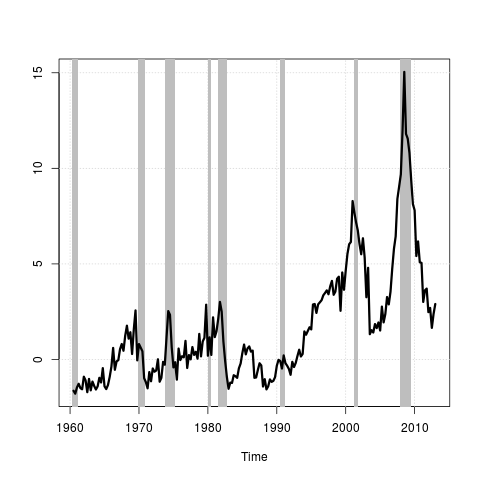
\includegraphics[scale=0.5]{./results/pics0.01/fpucoin.png} & 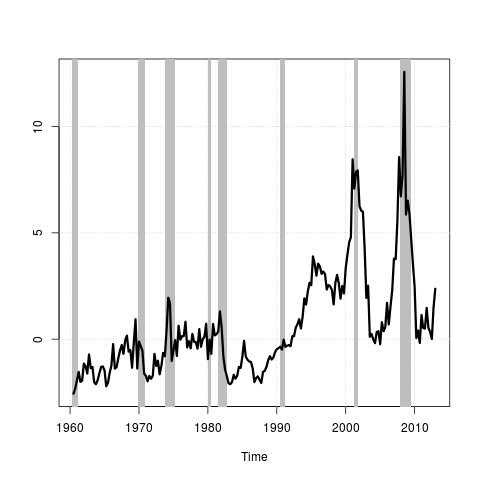
\includegraphics[scale=0.5]{./results/pics0.02/fpucoin.png} \\ 
Learning Gain = 0.01 & Learning Gain = 0.02 \\ 
\multicolumn{2}{c}{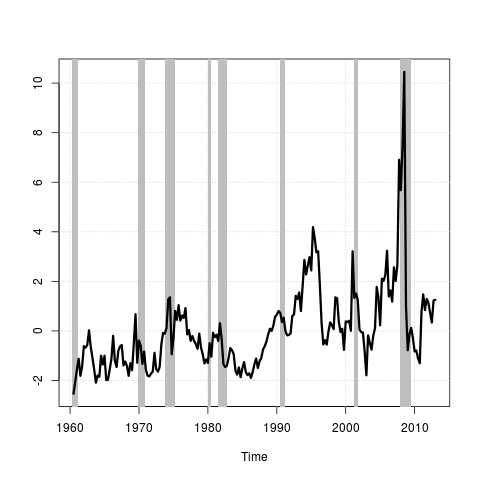
\includegraphics[scale=0.5]{./results/pics0.04/fpucoin.png}} \\
\multicolumn{2}{c}{Learning Gain = 0.04} 
\end{tabular}
\end{figure} 

I estimate equations (\ref{eq:measure}) through (\ref{eq:error}) by maximum likelihood and obtain smoothed estimates for the series $\lambda_t$ and $e_t$.  Plots of the coincident indicator for fiscal uncertainty are shown in Figure \ref{fg:fpucoin} for learning gains equal to 0.01, 0.02 and 0.04.  Again, the figure suggests relatively low fiscal uncertainty from 1960 through the middle to late 1980s.  There is a buildup of fiscal policy uncertainty beginning in the late 1980s or early 1990s, reaching peaks just preceding the recessions beginning in 2001 and 2007.  The different learning gains tell mostly the same qualitative story, but differ somewhat in magnitude.  The largest magnitude for fiscal uncertainty is predicted by the expectations framework with the lowest learning gain, which is expected.  Agents that use a smaller learning gain adjust their expectations more slowly in response to unexpected fiscal policy actions.  If these fiscal policy actions have persistence, they continue to be unexpected until agents learn the new behavior.  

\begin{figure}\caption{Unique Components of Fiscal Uncertainty}\label{fg:fpuremove0.02}
\begin{center}
\begin{tabular}{cc}
\multicolumn{2}{c}{Learning Gain = 0.02} \\ [0.5pc]
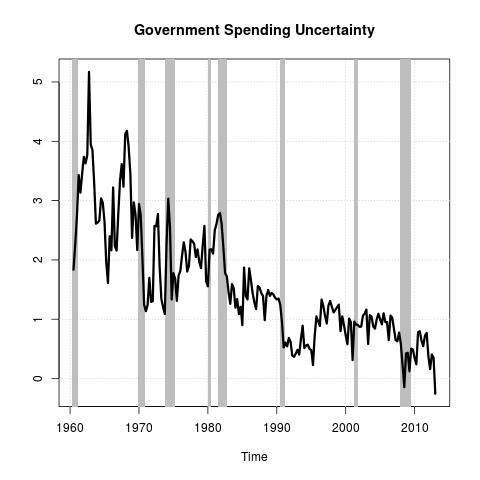
\includegraphics[scale=0.45]{./results/pics0.02/fpucoin_gov.png} & 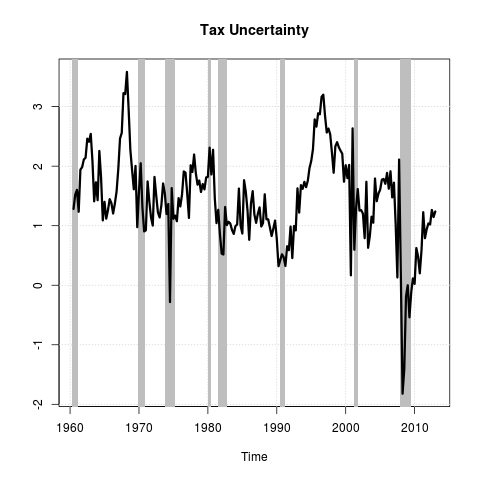
\includegraphics[scale=0.45]{./results/pics0.02/fpucoin_tax.png} \\
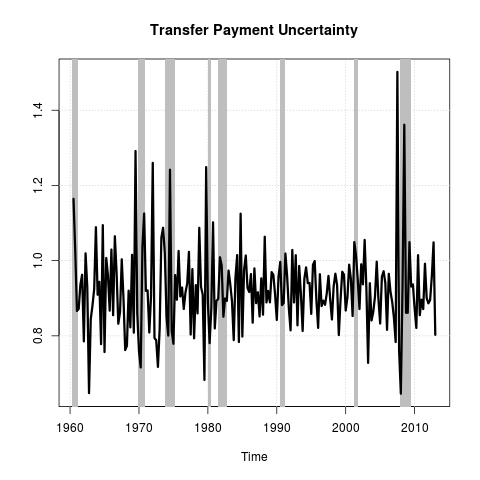
\includegraphics[scale=0.45]{./results/pics0.02/fpucoin_transfers.png} & 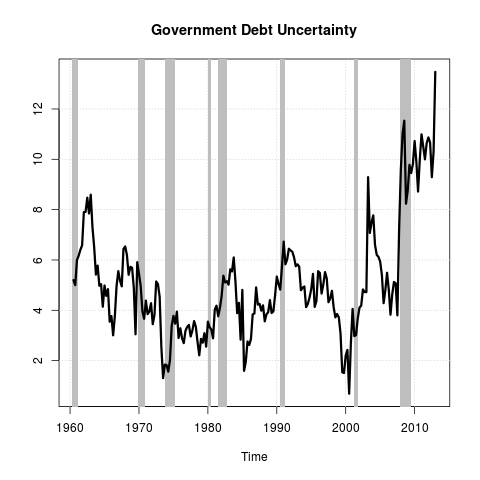
\includegraphics[scale=0.45]{./results/pics0.02/fpucoin_debt.png}  
\end{tabular}
\end{center}
\end{figure} 

Figure \ref{fg:fpuremove0.02} shows plots of the unique component of each fiscal uncertainty variable with a learning gain equal to 0.02.  Relative uncertainty on government spending has declined over time.  Relative uncertainty on taxes increased while tax revenue was increasing during the 1990s, but has fallen off since then.  The opposite can be said of relative uncertainty regarding government debt.  Here there was a decline during the 1990s when debt relative to real GDP was falling, but the relative uncertainty concerning government debt increased after 2000 and has remained high while at the same time the level of debt to GDP was rising and has remained high.  Transfers uncertainty closely follows the coincident fiscal uncertainty measure.  It can be seen that the common component of fiscal uncertainty in Figure \ref{fg:fpucoin} (when the learning gain is equal to 0.02) very closely resembles the original plot for transfers uncertainty in Figure \ref{fg:fpu0.02}.  As a consequence, the unique component for transfers is reduced to what appears to be a nearly independently and identically distributed stochastic process. 

The evolution for the unique components of fiscal uncertainty under alternative learning gains are discussed in the appendix and shown in Figures \ref{fg:fpuremove0.01} and \ref{fg:fpuremove0.04}.  Again, while the magnitudes for fiscal uncertainty differ across different learning gains, the direction and timing of the movements are all very similar.

Panel (b) of Table \ref{tb:fpucorrel0.02} shows the correlations of the unique components with each other.  Comparing panels (a) and (b) reveals that removing the common component of fiscal policy uncertainty leads to much lower correlation between each pair of fiscal variables.  Panel (c) of Table \ref{tb:fpucorrel0.02} shows how strongly correlated each unadjusted fiscal uncertainty variable is to the common component of fiscal uncertainty.  The correlations range from 0.75 to 0.99, indicating that all of the fiscal uncertainty variables are strongly correlated with the common component.  I repeat the exercise in this section with fiscal uncertainty variables constructed with alternative calibrations for the learning gain, and report the correlations in Tables \ref{tb:fpucorrel0.01} and \ref{tb:fpucorrel0.04}.  The magnitudes for the correlations differ only slightly with different learning gains. 

\begin{figure}\caption{Coincident Fiscal Uncertainty with Baker et. al. (2013) Policy Uncertainty}\label{fg:fpuindex}
\hspace*{-0.3in}\begin{tabular}{cc}
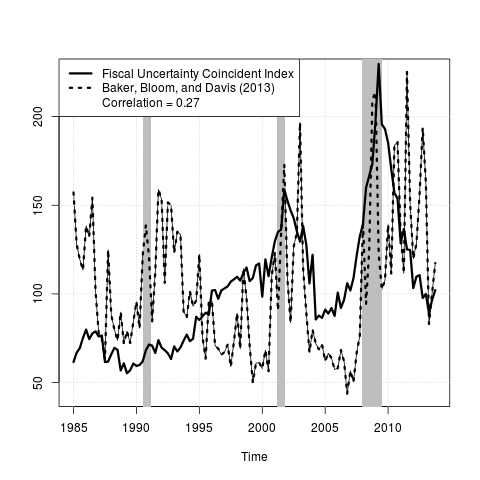
\includegraphics[scale=0.5]{./results/pics0.01/fpuindex.png} & 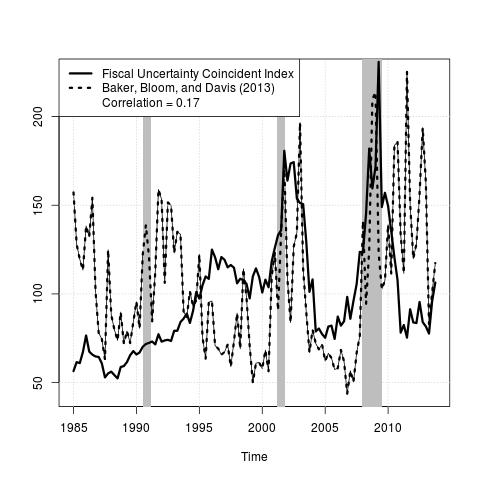
\includegraphics[scale=0.5]{./results/pics0.02/fpuindex.png} \\ 
Learning Gain = 0.01 & Learning Gain = 0.02 \\ 
\multicolumn{2}{c}{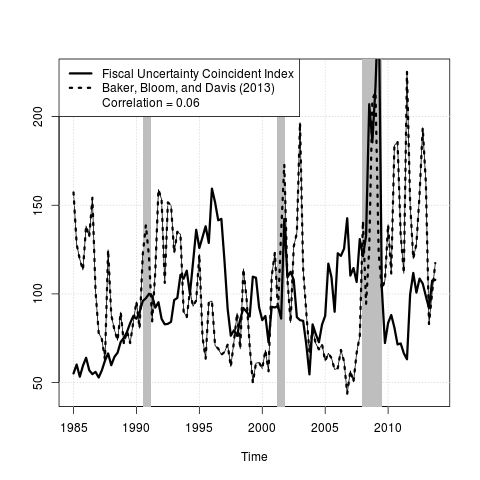
\includegraphics[scale=0.5]{./results/pics0.04/fpuindex.png}} \\
\multicolumn{2}{c}{Learning Gain = 0.04} 
\end{tabular}
\end{figure} 

The coincident indicator for fiscal uncertainty is similar in its purpose and meaning as the policy uncertainty index constructed by \citee{baker2013} (henceforth BBD index).  These authors construct an index of policy uncertainty that includes monetary and fiscal policy, and which is based on three factors: frequency of major newspaper headlines on the subject of policy uncertainty, number of existing tax policies that are soon due to expire, and the variance of professional forecasts for policy variables.  While the coincident indicator for fiscal uncertainty in the present paper differs significantly in its methodology from the BBD index, the measures are positively correlated; though the strength of the correlation depends on the learning gain.  Figure \ref{fg:fpuindex} shows plots that compare the BBD index (dotted line) with the common component for fiscal uncertainty (solid line) over the period 1985 through 2013, the period in which the BBD index is available.  The figure includes the estimated common component constructed for three different learning gains, including 0.01, 0.02, and 0.04.  The coincident indicators are re-scaled from what is shown in Figure \ref{fg:fpucoin} to match the scaling procedure that was used to construct the BBD index.  The coincident index is multiplied by a constant proportion so that the variance of the coincident index matches the variance of BBD over the sub-sample 1985 - 2009, and a constant is added so that mean of the coincident index is equal to 100.0 over the same sub-sample.

The correlation of each coincident indicator with the BBD index are also reported in Figure \ref{fg:fpuindex}.  The correlations are positive, but small, and are the largest with the smaller, more empirically plausible, learning gains.  The largest correlation is 0.27 with a learning gain equal to 0.01 and the smallest correlation is 0.06 with a learning gain equal to 0.04.  While there appears to be little relationship in the time series in the first half of the sample, the measures move more closely together over the last fifteen years of the sample.  There is a buildup of policy uncertainty beginning near 2000 which persists for a couple of years beyond the 2001 recession before coming back down.  Another larger buildup of fiscal uncertainty begins before the onset of the 2007-2009 recession and eventually comes back down by the end of the sample.  

While the BBD index and the coincident index for fiscal uncertainty in the present paper are similar in their purposes and meaning, there are a number of reasons to expect these measures may not be highly correlated.  First, the BBD index is more likely endogenously determined with the health of the macroeconomy, given that fiscal policy is more likely to make headline news when the economy is suffering from a recessionary gap.  The common component of fiscal uncertainty is less likely susceptible to this problem because the predicted values for fiscal variables use concurrent macroeconomic conditions among its explanatory variables.  The prediction errors from the regression that make up the measure for fiscal uncertainty are therefore not likely related to concurrent economic conditions.\footnote{The coincident index for fiscal uncertainty is still possibly endogenously determined with macroeconomic outcomes, if structural changes in the fiscal policy rules endogenously depend on economic conditions.  In such a case, the structural change leads to a larger prediction error, and therefore a larger degree of fiscal uncertainty.} Secondly, the BBD index includes a forward-looking aspect while the coincident index for fiscal uncertainty is purely backward looking.  The BBD index includes incorporates information on the number of tax laws that are due to expire.  The fiscal uncertainty measures constructed in this paper would only pick up this information after the expiration of the policy, and only insomuch that the expiration of the tax policy alters the aggregate behavior tax revenues or net transfers. 

\section{Macroeconomic Impact of Fiscal Uncertainty}

I now turn to estimating the effect that fiscal policy uncertainty has on the macroeconomy.  I estimate an autoregressive distributed lag models (ARDL) for several macroeconomic outcome variables, including real GDP, consumption, investment, employment, unemployment, and inflation, and include as explanatory variables the measures of fiscal policy uncertainty constructed in the previous section.  As above, the quantity variables real GDP, consumption, and investment are put in per-capita terms, and expressed as a ratio of the previous quarter's real GDP per capita.  Employment is given by the total number of employed persons from the Bureau of Labor Statistics.  It is also put in per-capita terms, and so is the employment to population ratio.  Unemployment is the civilian unemployment rate from the Bureau of Labor Statistics.  Finally, inflation is the annualized quarterly growth rate of the GDP Implicit Price Deflator from the Bureau of Economic Analysis.

\subsection{Regression Model}

Let $s_t$ denote the vector of macroeconomic variables above, and $s_t^i$ denote the time $t$ realization of one of variables of the vector.  The ARDL model to be estimated is given by,
\beq \label{eg:ardl} s_t^i = \Psi(L)s_t + \Phi(L)\tilde{f}_t + \Gamma \tilde{m}_{t-1} + \psi \lambda_{t-1} + \xi_t. \eeq
Here, $\Psi(L)$ is a distributed lag operator denoting the set of coefficient vectors for each lag of the macroeconomic controls.  The vector $\tilde{f}_t$ denotes a subset of the fiscal policy variables in $f_t$ from the previous section, namely government expenditures, tax revenue, and net transfers.  The operator $\Phi(L)$ is a distributed lag operator for the set of coefficients on each of these fiscal policy variables.  I assume identical lag lengths for $\Psi(L)$ and $\Phi(L)$.  The vector $\tilde{m}_{t-1}$ denotes the unique components of fiscal policy uncertainty at time $t-1$ and $\Gamma$ is the associated vector of coefficients.  The variable $\lambda_{t-1}$ is the common component of fiscal uncertainty and $\psi$ is the associated coefficient.  Finally, $\xi_t$ denotes the error term.  

\begin{table}\caption{Regression Results - Learning Gain = 0.02, Lag Length = 1}\label{tb:ARDL_1lags_0.02gain}\scriptsize{
\begin{center}\begin{tabular}{l|S[table-format=3.2] S[table-format=3.2] S[table-format=3.2] S[table-format=3.2] S[table-format=3.2] S[table-format=3.2]}
 & \multicolumn{1}{p{0.6in}}{\vspace*{-1.5pc}\begin{center}~\newline Real GDP\end{center}} 
                & \multicolumn{1}{p{0.6in}}{\vspace*{-1.5pc}\begin{center}Consumption\end{center}} 
                & \multicolumn{1}{p{0.6in}}{\vspace*{-1.5pc}\begin{center}~\newline Investment\end{center}} 
                & \multicolumn{1}{p{0.6in}}{\vspace*{-1.5pc}\begin{center}Employment\end{center}}
                & \multicolumn{1}{p{0.6in}}{\vspace*{-1.5pc}\begin{center}Unemployment\end{center}} 
                & \multicolumn{1}{p{0.6in}}{\vspace*{-1.5pc}\begin{center}~\newline Inflation\end{center}} \\ [-0.75pc] \hline
 & \multicolumn{6}{c}{} \\ [-0.25pc]
Fiscal Uncertainty Coefficients$^1$~~ & \multicolumn{6}{c}{} \\ [0.5pc]
~~~Government Expenditures & -0.04 & 0.10 & -0.10 & -0.72 & 0.41*** & 0.01 \\
~~~(Standard Error) & (0.10) & (0.07) & (0.07) & (0.89) & (0.16) & (0.21) \\ [0.2pc]
~~~Tax Receipts & 0.32*** & 0.03 & 0.32*** & 0.26 & -0.08 & 0.03 \\
~~~(Standard Error) & (0.10) & (0.05) & (0.06) & (0.25) & (0.13) & (0.14) \\ [0.2pc]
~~~Transfer Payments & 0.11** & 0.00 & 0.08** & -0.25 & -0.01 & 0.08 \\
~~~(Standard Error) & (0.05) & (0.03) & (0.04) & (0.53) & (0.06) & (0.12) \\ [0.2pc]
~~~Government Debt & 0.06 & -0.06 & 0.13* & -1.09* & 0.23 & 0.21 \\
~~~(Standard Error) & (0.09) & (0.06) & (0.07) & (0.65) & (0.18) & (0.15) \\ [0.2pc]
~~~Coincident Index & -0.43*** & -0.22*** & -0.25*** & 0.36 & -0.34*** & -0.28*** \\
~~~(Standard Error) & (0.10) & (0.04) & (0.08) & (1.17) & (0.11) & (0.10) \\ [0.2pc]
\hline
 & \multicolumn{6}{c}{} \\ [-0.25pc]
Fiscal Uncertainty Joint Wald$^2$~~ & 5.64*** & 6.52*** & 5.90*** & 3.04** & 5.28*** & 2.11* \\ [0.5pc] \hline
 & \multicolumn{6}{c}{} \\ [-0.25pc]
Wald Tests for Controls$^3$ & \multicolumn{6}{c}{} \\ [0.5pc]
~~~Real GDP & 17.19*** & 24.59*** & 8.82*** & 0.10 & 9.57*** & 7.29*** \\
~~~Consumption & 8.95*** & 183.81*** & 0.71 & 0.03 & 1.43 & 0.45 \\
~~~Investment & 0.67 & 465.17*** & 5.06** & 0.03 & 0.42 & 1.02 \\
~~~Employment & 13.09*** & 0.37 & 122.86*** & 0.78 & 8.50*** & 1.60 \\
~~~Unemployment & 7.06*** & 18.63*** & 3.29* & 0.22 & 2.80* & 82.94*** \\
~~~Inflation & 6.50** & 0.00 & 8.83*** & 0.03 & 0.23 & 1.30 \\
~~~Government Expenditures & 1.34 & 11.85*** & 2.42 & 0.08 & 7.07*** & 0.14 \\
~~~Transfer Payments & 4.12** & 1.18 & 2.83* & 0.19 & 4.41** & 0.24 \\
~~~Tax Receipts & 10.21*** & 11.66*** & 16.57*** & 0.15 & 12.19*** & 12.32*** \\


\hline
 & \multicolumn{6}{c}{} \\ [-0.25pc]
Fit Statistics: & \multicolumn{6}{c}{} \\ [0.5pc]
~~~Adjusted R-square & 0.25 & 0.98 & 0.95 & 0.82 & 0.84 & 0.80 \\
~~~AIC & 480.01 & 193.75 & 294.88 & 675.85 & 427.47 & 637.55 \\
~~~BIC & 533.56 & 247.30 & 348.43 & 729.40 & 481.03 & 691.10 \\ \hline
\multicolumn{7}{p{6in}}{
                1. Standard errors are Newey West heteroskedastic and autocorrelation robust.\newline
                2. Null hypothesis: Coefficients on all fiscal uncertainty variables are equal to zero. Wald F-test $\sim$ F(5,195).\newline
                3. Null hypothesis: All 1 lags of the given control variable have coefficients equal to zero. Wald F-test $\sim$ F(1,195).\newline
                * Significant at 10\% level~~ ** Significant at 5\% level~~ *** Significant at 1\% level}
\end{tabular}\end{center}}\end{table}

\begin{table}\caption{Regression Results - Learning Gain = 0.02, Lag Length = 2}\label{tb:ARDL_2lags_0.02gain}\scriptsize{
\begin{center}\begin{tabular}{l|S[table-format=3.2] S[table-format=3.2] S[table-format=3.2] S[table-format=3.2] S[table-format=3.2] S[table-format=3.2]}
 & \multicolumn{1}{p{0.6in}}{\vspace*{-1.5pc}\begin{center}~\newline Real GDP\end{center}} 
                & \multicolumn{1}{p{0.6in}}{\vspace*{-1.5pc}\begin{center}Consumption\end{center}} 
                & \multicolumn{1}{p{0.6in}}{\vspace*{-1.5pc}\begin{center}~\newline Investment\end{center}} 
                & \multicolumn{1}{p{0.6in}}{\vspace*{-1.5pc}\begin{center}Employment\end{center}}
                & \multicolumn{1}{p{0.6in}}{\vspace*{-1.5pc}\begin{center}Unemployment\end{center}} 
                & \multicolumn{1}{p{0.6in}}{\vspace*{-1.5pc}\begin{center}~\newline Inflation\end{center}} \\ [-0.75pc] \hline
 & \multicolumn{6}{c}{} \\ [-0.25pc]
Fiscal Uncertainty Coefficients$^1$~~ & \multicolumn{6}{c}{} \\ [0.5pc]
~~~Government Expenditures & -0.04 & 0.06 & -0.06 & -0.68** & 0.55*** & 0.02 \\
~~~(Standard Error) & (0.11) & (0.07) & (0.08) & (0.28) & (0.13) & (0.25) \\ [0.2pc]
~~~Tax Receipts & 0.36*** & 0.07 & 0.26*** & 0.39 & -0.22 & 0.05 \\
~~~(Standard Error) & (0.11) & (0.06) & (0.09) & (0.28) & (0.14) & (0.15) \\ [0.2pc]
~~~Transfer Payments & -0.01 & -0.03 & 0.01 & -0.49** & 0.19*** & 0.01 \\
~~~(Standard Error) & (0.08) & (0.04) & (0.04) & (0.23) & (0.06) & (0.12) \\ [0.2pc]
~~~Government Debt & 0.05 & -0.03 & 0.09 & -1.27 & 0.25 & 0.12 \\
~~~(Standard Error) & (0.10) & (0.06) & (0.06) & (0.88) & (0.16) & (0.17) \\ [0.2pc]
~~~Coincident Index & -0.41*** & -0.21*** & -0.19*** & 0.13 & -0.22* & -0.36** \\
~~~(Standard Error) & (0.10) & (0.05) & (0.07) & (0.38) & (0.14) & (0.16) \\ [0.2pc]
\hline
 & \multicolumn{6}{c}{} \\ [-0.25pc]
Fiscal Uncertainty Joint Wald$^2$~~ & 4.02*** & 3.80*** & 2.54** & 3.21*** & 4.27*** & 1.29 \\ [0.5pc] \hline
 & \multicolumn{6}{c}{} \\ [-0.25pc]
Wald Tests for Controls$^3$ & \multicolumn{6}{c}{} \\ [0.5pc]
~~~Real GDP & 8.90*** & 13.45*** & 5.34*** & 1.53 & 5.33*** & 5.75*** \\
~~~Consumption & 16.58*** & 39.94*** & 10.03*** & 0.46 & 1.67 & 0.35 \\
~~~Investment & 9.51*** & 212.55*** & 14.30*** & 0.30 & 0.61 & 1.16 \\
~~~Employment & 11.97*** & 1.71 & 62.87*** & 0.91 & 5.54*** & 1.39 \\
~~~Unemployment & 2.98* & 7.02*** & 2.13 & 0.43 & 0.96 & 34.67*** \\
~~~Inflation & 4.87*** & 0.71 & 3.93** & 1.27 & 3.71** & 0.69 \\
~~~Government Expenditures & 5.41*** & 6.32*** & 2.05 & 4.51** & 10.25*** & 0.85 \\
~~~Transfer Payments & 4.19** & 1.09 & 2.30 & 1.11 & 3.34** & 0.57 \\
~~~Tax Receipts & 3.69** & 4.16** & 5.29*** & 0.87 & 4.45** & 5.30*** \\


\hline
 & \multicolumn{6}{c}{} \\ [-0.25pc]
Fit Statistics: & \multicolumn{6}{c}{} \\ [0.5pc]
~~~Adjusted R-square & 0.32 & 0.98 & 0.96 & 0.83 & 0.87 & 0.81 \\
~~~AIC & 466.15 & 198.35 & 257.72 & 666.99 & 398.54 & 632.69 \\
~~~BIC & 549.83 & 282.03 & 341.40 & 750.67 & 482.22 & 716.37 \\ \hline
\multicolumn{7}{p{6in}}{
                1. Standard errors are Newey West heteroskedastic and autocorrelation robust.\newline
                2. Null hypothesis: Coefficients on all fiscal uncertainty variables are equal to zero. Wald F-test $\sim$ F(5,186).\newline
                3. Null hypothesis: All 2 lags of the given control variable have coefficients equal to zero. Wald F-test $\sim$ F(2,186).\newline
                * Significant at 10\% level~~ ** Significant at 5\% level~~ *** Significant at 1\% level}
\end{tabular}\end{center}}\end{table}

\begin{table}\caption{Regression Results - Learning Gain = 0.02, Lag Length = 4}\label{tb:ARDL_4lags_0.02gain}\scriptsize{
\begin{center}\begin{tabular}{l|S[table-format=3.2] S[table-format=3.2] S[table-format=3.2] S[table-format=3.2] S[table-format=3.2] S[table-format=3.2]}
 & \multicolumn{1}{p{0.6in}}{\vspace*{-1.5pc}\begin{center}~\newline Real GDP\end{center}} 
                & \multicolumn{1}{p{0.6in}}{\vspace*{-1.5pc}\begin{center}Consumption\end{center}} 
                & \multicolumn{1}{p{0.6in}}{\vspace*{-1.5pc}\begin{center}~\newline Investment\end{center}} 
                & \multicolumn{1}{p{0.6in}}{\vspace*{-1.5pc}\begin{center}Employment\end{center}}
                & \multicolumn{1}{p{0.6in}}{\vspace*{-1.5pc}\begin{center}Unemployment\end{center}} 
                & \multicolumn{1}{p{0.6in}}{\vspace*{-1.5pc}\begin{center}~\newline Inflation\end{center}} \\ [-0.75pc] \hline
 & \multicolumn{6}{c}{} \\ [-0.25pc]
Fiscal Uncertainty Coefficients$^1$~~ & \multicolumn{6}{c}{} \\ [0.5pc]
~~~Government Expenditures & -0.13 & 0.03 & -0.08 & -0.58 & 0.47*** & 0.09 \\
~~~(Standard Error) & (0.12) & (0.06) & (0.08) & (0.39) & (0.13) & (0.23) \\ [0.2pc]
~~~Tax Receipts & 0.43*** & 0.03 & 0.30*** & 0.35 & -0.17 & 0.02 \\
~~~(Standard Error) & (0.11) & (0.06) & (0.07) & (0.38) & (0.13) & (0.20) \\ [0.2pc]
~~~Transfer Payments & -0.01 & -0.04 & 0.02 & -0.45*** & 0.18*** & 0.04 \\
~~~(Standard Error) & (0.08) & (0.05) & (0.04) & (0.17) & (0.05) & (0.12) \\ [0.2pc]
~~~Government Debt & 0.15 & -0.01 & 0.15*** & -1.20 & 0.26* & 0.03 \\
~~~(Standard Error) & (0.10) & (0.06) & (0.05) & (0.95) & (0.15) & (0.19) \\ [0.2pc]
~~~Coincident Index & -0.40*** & -0.12* & -0.21*** & 0.04 & -0.21 & -0.47* \\
~~~(Standard Error) & (0.10) & (0.06) & (0.06) & (0.41) & (0.15) & (0.24) \\ [0.2pc]
\hline
 & \multicolumn{6}{c}{} \\ [-0.25pc]
Fiscal Uncertainty Joint Wald$^2$~~ & 4.44*** & 1.06 & 4.86*** & 1.65 & 5.54*** & 1.53 \\ [0.5pc] \hline
 & \multicolumn{6}{c}{} \\ [-0.25pc]
Wald Tests for Controls$^3$ & \multicolumn{6}{c}{} \\ [0.5pc]
~~~Real GDP & 8.89*** & 4.71*** & 12.48*** & 1.03 & 4.20*** & 1.92 \\
~~~Consumption & 3.32** & 18.01*** & 4.36*** & 0.36 & 2.08* & 2.31* \\
~~~Investment & 5.19*** & 87.23*** & 5.04*** & 0.18 & 0.53 & 3.74*** \\
~~~Employment & 6.17*** & 0.30 & 35.01*** & 0.87 & 3.82*** & 1.39 \\
~~~Unemployment & 3.23** & 2.37* & 2.45** & 0.45 & 0.17 & 13.35*** \\
~~~Inflation & 3.49*** & 0.65 & 4.61*** & 2.01* & 6.20*** & 0.41 \\
~~~Government Expenditures & 4.25*** & 2.20* & 1.43 & 2.54** & 7.00*** & 3.67*** \\
~~~Transfer Payments & 4.91*** & 1.30 & 3.77*** & 0.45 & 1.74 & 1.15 \\
~~~Tax Receipts & 4.15*** & 1.54 & 6.33*** & 0.48 & 2.88** & 2.59** \\


\hline
 & \multicolumn{6}{c}{} \\ [-0.25pc]
Fit Statistics: & \multicolumn{6}{c}{} \\ [0.5pc]
~~~Adjusted R-square & 0.39 & 0.98 & 0.96 & 0.84 & 0.89 & 0.82 \\
~~~AIC & 459.08 & 203.62 & 254.38 & 679.46 & 378.98 & 631.62 \\
~~~BIC & 603.00 & 347.55 & 398.30 & 823.38 & 522.91 & 775.55 \\ \hline
\multicolumn{7}{p{6in}}{
                1. Standard errors are Newey West heteroskedastic and autocorrelation robust.\newline
                2. Null hypothesis: Coefficients on all fiscal uncertainty variables are equal to zero. Wald F-test $\sim$ F(5,168).\newline
                3. Null hypothesis: All 4 lags of the given control variable have coefficients equal to zero. Wald F-test $\sim$ F(4,168).\newline
                * Significant at 10\% level~~ ** Significant at 5\% level~~ *** Significant at 1\% level}
\end{tabular}\end{center}}\end{table}


This set of ARDL equations is rich in explanatory variables.  The purpose for this is to estimate the channel for which fiscal uncertainty may influence the macroeconomy, while allowing for complex macroeconomic dynamics.  This includes allowing fiscal policy to directly influence the macroeconomy with the inclusion of $\Phi(L) \tilde{f}_{t}$, and allowing the six macroeconomic variables to influence each other over time with the inclusion of $\Psi(L)s_t$.  I estimate the ARDL model for the six macroeconomic variables above, with different lengths.  Tables \ref{tb:ARDL_1lags_0.02gain}, \ref{tb:ARDL_2lags_0.02gain}, and \ref{tb:ARDL_4lags_0.02gain} show the regression results when uncertainty is computed using a learning gain equal to 0.02 and using distributed lag lengths equal to 1, 2, and 4, respectively.  The top part of the tables report the estimated coefficients on the fiscal uncertainty variables and their standard errors (Newey-West heteroskedastic and autocorrelation robust).  With every lag specification, the results show that the common component of fiscal policy uncertainty leads to statistically significant decreases in real GDP, consumption, and investment.  The coefficient on inflation is also negative and statistically significant in each specification, indicating that fiscal uncertainty leads to a decrease in inflation.  This is contrary to the theoretical finding by \citee{fvetal2011}, who use a calibrated New Keynesian business cycle model to demonstrate that fiscal uncertainty can have stagflationary effects.  Rather, it appears that fiscal uncertainty causes a drag on aggregate demand that pushes consumption spending, investment spending, real GDP, and the rate of inflation downward.  

The coefficient on unemployment rate is negative in each case, but only statistically significant at the 5\% level in one specification and the coefficient on the employment / population ratio is positive, but never statistically significant.  This could be due to a labor supply effect.  Recall that the common component for fiscal uncertainty is nearly perfectly correlated with the unadjusted estimate for government transfers uncertainty.  Greater uncertainty on future payouts, possibly from social welfare programs such as unemployment insurance or nutritional assistance programs, may lead unemployed people to put forward more effort into obtaining employment.  \citee{FarberValletta} find some limited statistical evidence in support of such a theory.  They find that the unemployment rate and the average unemployment duration both increase in response to an extension of unemployment benefits, which can be viewed as a decrease in uncertainty, but the magnitudes that they find are small.  Moreover, they attribute most of this increase in unemployment not to a reduction in the job-finding rate, but a reduction in the labor-supply exit rate.

The coefficients reveal another robust finding that uncertainty regarding tax revenue, specifically, leads to statistically significant increases in investment and real GDP.  \citee{born2011} offer competing explanations for opposing effects that policy uncertainty can have on investment.  In one case, subject to greater uncertainty, investment decisions are postponed until times are more certain, therefore depressing investment.  On the other hand, firms that are risk averse self insure in the presence of greater uncertainty by building up a buffer capital stock.  Also, consumers that are risk averse supply more labor when subject to greater uncertainty.  The increase in employment leads to an increase in the marginal product of capital, which also boosts investment demand.  The empirical results in the present paper suggest the latter effect dominates when it comes to uncertainty specifically concerning taxes.  Subject to general fiscal uncertainty, the former effect dominates.

Given there are five fiscal uncertainty variables in the empirical model, I estimate a joint Wald test with the null hypothesis that the coefficients on all the fiscal uncertainty coefficients are equal to zero.  In nearly every case, the test is strongly rejected. Therefore uncertainty regarding one or more fiscal policy variables does indeed have statistically significant effects on a number of macroeconomic outcomes.  An exception is the regression on inflation, which is not statistically significant at the longer lag lengths, and it is only significant at the 10\% level with lag length equal to one quarter.  Also, at lag length equal to four quarters, the joint Wald is not statistically significant for consumption and employment, likely due to diminished degrees of freedom (given the long lag length on numerous controls, these regressions contain 41 explanatory variables).

Rather than reporting the estimated coefficients for the long list of controls, each with multiple lags, Tables \ref{tb:ARDL_1lags_0.02gain}, \ref{tb:ARDL_2lags_0.02gain}, and \ref{tb:ARDL_4lags_0.02gain} report joint Wald statistics for each set of controls.  The null hypothesis for a given control variable is that the coefficients on all the lags of that variable are equal to zero.  Many of these are statistically significant, so it is likely important to include these macroeconomic and fiscal policy control variables to account for complex macroeconomic dynamics and dependence while finding evidence for the impact of fiscal uncertainty.

To check for robustness, in the appendix I repeat this regression analysis using fiscal uncertainty constructed from alternative calibrations for the learning gain.  

\subsection{Magnitude of the Impact}\label{s:impact}

The magnitude of the regression coefficients may suggest that fiscal uncertainty is not a quantitatively important driver of business cycles.  Take, for example, the regression coefficients on the common component of fiscal uncertainty in the ARDL regression with two lags (Table \ref{tb:ARDL_2lags_0.02gain}).  The common component for fiscal uncertainty is an index with a standard deviation normalized to 1.0.  The regression coefficient for real GDP is statistically significantly negative, and equal to -0.41, which implies a one-standard deviation increase in the common component of fiscal uncertainty leads to a 0.4\% decline in real GDP.  While this magnitude is not negligible, it may not appear to be evidence that fiscal uncertainty is a primary driver of business cycles or a leading factor explaining the Great Recession or subsequent slow recovery.  \citee{fvetal2011} suggest that while normal fluctuations in policy uncertainty may not be quantitatively important for macroeconomic dynamics, the once-in-a-decade spike in policy uncertainty should be of concern.  \citee{baker2013} also speak to the quantitative importance of a long-horizon buildup of policy uncertainty, finding that the growth policy uncertainty from 2006 to 2011 was associated with a 2.5\% decline in industrial production and a 2.3 million person decline in total employment.

%%%%%%%%%%%%%%%%%%%%%%%%%%%%%%%%%%%%%%%%%%%%%%%%%%%%%%%%%%%%%%%%%%%%%%%%%%%%%%%%%%%%%%%%%%%%%%%%%%%%%%%%%%%%%
\begin{table}\caption{Impact from an Extreme Decade of Fiscal Uncertainty}\label{tb:impact_0.02gain}\footnotesize{
\begin{center}
\subcaption{Magnitude of Extreme Change in Coincident Fiscal Uncertainty (Learning Gain = 0.02)}
\begin{tabular}{l|S[table-format=3.2] S[table-format=3.2] S[table-format=3.2] S[table-format=3.2]} \hline
\multicolumn{3}{l}{Largest Value Coincident Fiscal Uncertainty = 4.77} & \multicolumn{1}{r}{Date: 2009 Quarter 2} & \\
\multicolumn{3}{l}{Smallest Value in Decade Preceding = -0.34} & \multicolumn{1}{r}{Date: 2005 Quarter 4} & \\ \hline
\end{tabular}
\ \\ \ \\ \ \\

\subcaption{Estimates using ARDL with 1 Lag}
\begin{tabular}{l|S[table-format=3.2] S[table-format=3.2] S[table-format=3.2] S[table-format=3.2]}
 \multicolumn{1}{p{1in}}{Variable} 
                & \multicolumn{1}{p{1in}}{\vspace*{-1.5pc}\begin{center}Coefficient\end{center}} 
                & \multicolumn{1}{p{1in}}{\vspace*{-1.5pc}\begin{center}Impact\end{center}} 
                & \multicolumn{1}{p{1in}}{\vspace*{-1.5pc}\begin{center}95\% Lower Bound\end{center}} 
                & \multicolumn{1}{p{1in}}{\vspace*{-1.5pc}\begin{center}95\% Upper Bound\end{center}}\\ [-0.75pc] \hline
Real GDP & -0.43*** & -2.19 & -3.22 & -1.15 \\
Consumption & -0.22*** & -1.12 & -1.57 & -0.68 \\
Investment & -0.25*** & -1.26 & -2.09 & -0.43 \\
Employment & 0.36 & 1.86 & -9.87 & 13.59 \\
Unemployment & -0.34*** & -1.73 & -2.83 & -0.64 \\
Inflation & -0.28*** & -1.43 & -2.46 & -0.39 \\
\hline
\end{tabular}
\ \\ \ \\ \ \\ \ \\

\subcaption{Estimates using ARDL with 2 Lags}
\begin{tabular}{l|S[table-format=3.2] S[table-format=3.2] S[table-format=3.2] S[table-format=3.2]}
 \multicolumn{1}{p{1in}}{Variable} 
                & \multicolumn{1}{p{1in}}{\vspace*{-1.5pc}\begin{center}Coefficient\end{center}} 
                & \multicolumn{1}{p{1in}}{\vspace*{-1.5pc}\begin{center}Impact\end{center}} 
                & \multicolumn{1}{p{1in}}{\vspace*{-1.5pc}\begin{center}95\% Lower Bound\end{center}} 
                & \multicolumn{1}{p{1in}}{\vspace*{-1.5pc}\begin{center}95\% Upper Bound\end{center}}\\ [-0.75pc] \hline
Real GDP & -0.41*** & -2.07 & -3.04 & -1.11 \\
Consumption & -0.21*** & -1.06 & -1.57 & -0.54 \\
Investment & -0.19*** & -0.96 & -1.64 & -0.29 \\
Employment & 0.13 & 0.65 & -3.15 & 4.45 \\
Unemployment & -0.22* & -1.14 & -2.49 & 0.21 \\
Inflation & -0.36** & -1.85 & -3.50 & -0.20 \\
\hline
\end{tabular}
\ \\ \ \\ \ \\ \ \\

\subcaption{Estimates using ARDL with 4 Lags}
\begin{tabular}{l|S[table-format=3.2] S[table-format=3.2] S[table-format=3.2] S[table-format=3.2]}
 \multicolumn{1}{p{1in}}{Variable} 
                & \multicolumn{1}{p{1in}}{\vspace*{-1.5pc}\begin{center}Coefficient\end{center}} 
                & \multicolumn{1}{p{1in}}{\vspace*{-1.5pc}\begin{center}Impact\end{center}} 
                & \multicolumn{1}{p{1in}}{\vspace*{-1.5pc}\begin{center}95\% Lower Bound\end{center}} 
                & \multicolumn{1}{p{1in}}{\vspace*{-1.5pc}\begin{center}95\% Upper Bound\end{center}}\\ [-0.75pc] \hline
Real GDP & -0.40*** & -2.07 & -3.08 & -1.05 \\
Consumption & -0.12* & -0.60 & -1.24 & 0.03 \\
Investment & -0.21*** & -1.06 & -1.69 & -0.43 \\
Employment & 0.04 & 0.19 & -3.95 & 4.32 \\
Unemployment & -0.21 & -1.09 & -2.57 & 0.38 \\
Inflation & -0.47* & -2.40 & -4.82 & 0.02 \\
\hline
\multicolumn{5}{l}{* P-value < 0.10,~~~ ** P-value < 0.05,~~~ *** P-value < 0.01}
\end{tabular}

\end{center}}\end{table}
%%%%%%%%%%%%%%%%%%%%%%%%%%%%%%%%%%%%%%%%%%%%%%%%%%%%%%%%%%%%%%%%%%%%%%%%%%%%%%%%%%%%%%%%%%%%%%%%%%%%%%%%%%%%%

I provide some statistics in Table \ref{tb:impact_0.02gain} that speak to the macroeconomic impact that a decade-long buildup of fiscal uncertainty can have.  With every learning gain, the common component of fiscal uncertainty reaches its highest point in the sample in the second quarter of 2009, the last quarter of the Great Recession according to NBER official recession dating.  I search the preceding 10 years and find the lowest value that the common component of fiscal uncertainty took during that time.  For fiscal uncertainty computed using a learning gain equal to 0.02, this occurred in the fourth quarter of 2005.  I take the difference between these highest and lowest values, and multiply this by the ARDL coefficient on the common component of fiscal uncertainty to determine the magnitude that a large and long buildup of fiscal uncertainty can have on the macroeconomy.  Panels (b), (c) and (d) in Table \ref{tb:impact_0.02gain} report again the coefficients on the common component from the previous tables, the point estimates for the effects on the dependent variables from a large buildup in the common component of fiscal uncertainty, and a 95\% confidence interval of these effects, for ARDL specifications with 1, 2, and 4 lags, respectively.  The results for each lag specification are quantitatively similar.  The confidence intervals indicate that the buildup of fiscal uncertainty from late 2005 to mid 2009 led to a 1\% to 3\% decline in real GDP, which is in line with estimate by \cite{baker2013}.  A decline in consumption up to 1.5\% of lagged real GDP, and a decline in investment up to 2\% of lagged real GDP.  In the appendix, I provide some further discussion using fiscal uncertainty measures constructed using alternative learning gains.  In most cases, the magnitudes and evidence for statistical significant are similar.

\section{Conclusion}

Supposing that market participants form expectations on the behavior of fiscal policy by estimating simple regressions, I compute and describe the implied paths for fiscal uncertainty for four policy variables including government expenditures, taxes, transfers, and government debt.  From these measures, I compute a coincident indicator which provides a measure for a common component of fiscal policy uncertainty.  Using these measures of fiscal uncertainty in autoregressive distributed lag models, I demonstrate the macroeconomic consequences for fiscal uncertainty includes lower real GDP, consumption, and investment.  For the buildup of fiscal uncertainty that occurred in the years leading to the Great Recession, the magnitude of the impact on real GDP is sizable enough to help explain the severity of the Great Recession and subsequent slow recovery.

\nocite{*}
\begin{singlespace}
\bibliographystyle{apalike}
\bibliography{fiscaluncertainty}
\end{singlespace}

\newpage
\appendix
\section{Appendix} 

Here I explore how robust the findings in the paper are to alternative calibrations for the learning gain equal to 0.01 and 0.04.  The main content of this paper uses 0.02 as a learning gain, which is consistent with tightly estimated values in \citee{milani2007} and \citee{slobodyan_wouters_2012}.  The larger is the learning gain, the more weight is given to recent observations relative to older observations.  A larger learning gain leads to faster learning subject to a structural change in the data generating process, but it also subjects market participants to greater swings in expectations when subject to independent stochastic shocks, something that would not alter rational expectations.  

\subsection{Expectations and Uncertainty}
In Section \ref{s:common}, I construct market participants expectations and degrees of uncertainty using a learning gain equal to 0.02.  Here, I construct these measures again, using learning gains equal 0.01 and 0.04.  Figures \ref{fg:forecasts0.01} and \ref{fg:fe0.01} show the paths of expectations for each fiscal variable and the prediction errors using a learning gain equal to 0.01.  Figure \ref{fg:fpu0.01} shows the path for fiscal uncertainty based on the mean squared prediction error.  This exercise is repeated for a learning gain equal to 0.04 if Figures \ref{fg:forecasts0.04}, \ref{fg:fe0.04}, and \ref{fg:fpu0.04}.  While the magnitudes for the forecast errors and fiscal uncertainty differ between these learning gains, and differ from the magnitudes using a learning gain equal to 0.02 (Figures \ref{fg:fe0.02}, and \ref{fg:fpu0.02} discussed in the main part of the paper), the timing and direction of the movements in these variables are similar.  The difference in magnitude is to be expected.  Larger is the learning gains lead to greater swings in expectations, which lead to larger degrees of fiscal uncertainty.  The timing for the movements in fiscal uncertainty differ somewhat.  Because the larger learning gains lead to faster learning, for a learning gain equal to 0.04, the degree of fiscal uncertainty drops back to normal levels more quickly following spikes or buildups, as compared to learning gains equal to 0.01 or 0.02.

\subsection{Common Component of Fiscal Uncertainty}

Using a learning gain equal to 0.02, I show in Section \ref{s:common} that the resulting measures for uncertainty for the fiscal variables are highly correlated.  Panel (a) in each Table \ref{tb:fpucorrel0.01} and \ref{tb:fpuorrel0.04} confirm that this is also true when using learning gains equal to 0.01 and 0.04, respectively.  I estimate again the common component using the coincident indicator method described in Section \ref{s:common}, and when the common component is removed from the fiscal uncertainty variables, again they are much less strongly correlated, as panel (b) in each table reveals.  Finally, panel (c) in these tables reveals that the common component is highly correlated with all of the unadjusted fiscal uncertainty variables.  Figures \ref{fg:fpuremove0.01} and \ref{fg:fpuremove0.04} show the paths for the unique components of fiscal uncertainty for learning gains 0.01 and 0.04, respectively.

\subsection{Regression Results and Impact}
Tables \ref{tb:ARDL_1lags_0.01gain}, \ref{tb:ARDL_2lags_0.01gain}, and \ref{tb:ARDL_4lags_0.01gain} show the ARDL model results for lag lengths equal to 1, 2, and 4, respectively, when using fiscal uncertainty measures constructed from a learning gain equal to 0.01.  The exercise is repeated for a learning gain equal to 0.04 in Tables \ref{tb:ARDL_1lags_0.04gain}, \ref{tb:ARDL_2lags_0.04gain}, and \ref{tb:ARDL_4lags_0.04gain}.  In most cases, the signs and magnitudes on the regression coefficients on the common component of fiscal uncertainty are similar, and statistical significance appears in many of the same cases.  The largest exception is the ARDL model with lag length equal to four quarters and a learning gain equal to 0.04.  In this case there is little statistical evidence that the common component of fiscal uncertainty has macroeconomic effects.  This lack of robustness is not very troubling, as that learning gain is arguably farthest from what is empirically plausible.  Also, the model may suffer from too few degrees of freedom, as the ARDL with four lags on nine control variables leads to a model with 41 explanatory variables, including the five fiscal uncertainty variables.

Finally, Tables \ref{tb:impact_0.01gain} and \ref{tb:impact_0.04gain} show the estimated impact of the long-term extreme buildup of fiscal uncertainty that occurred during the Great Recession and the decade preceding it, using a learning gain equal to 0.01 and 0.04, respectively.  The estimates are similar to that using a learning gain equal to 0.02, which is discussed in Section \ref{s:impact} and presented in Table \ref{tb:impact_0.02gain}.  The only exception again are the results using a learning gain equal to 0.04 and lag length equal to four quarters, where the estimated effects are smaller, and are not precisely estimated.

%%%%%%%%%%%%%%%%%%%
% Appendix Tables %
%%%%%%%%%%%%%%%%%%%

\renewcommand*\thetable{A\arabic{table}}
\setcounter{table}{0}

\begin{table}[t]\caption{Fiscal Policy Uncertainty Correlations (Learning Gain = 0.01)}\label{tb:fpucorrel0.01}
\begin{center}
\subcaption{Fiscal Uncertainty Defined as Root Weighted Mean Squared Error}
\begin{tabular}{l|cccc}
 & Gov Spending & Tax Revenue & Transfers & Government Debt \\ \hline
Gov Spending & 1.00 & - & - & - \\
Tax Revenue & 0.44 & 1.00 & - & - \\
Transfers & 0.40 & 0.62 & 1.00 & - \\
Government Debt & 0.28 & 0.38 & 0.82 & 1.00 \\ \hline
\end{tabular}

\ \\ \ \\
\subcaption{Fiscal Uncertainty with Common Component Removed}
\begin{tabular}{l|cccc}
 & Gov Spending & Tax Revenue & Transfers & Government Debt \\ \hline
Gov Spending & 1.00 & - & - & - \\
Tax Revenue & 0.24 & 1.00 & - & - \\
Transfers & -0.12 & -0.14 & 1.00 & - \\
Government Debt & -0.32 & -0.35 & -0.12 & 1.00 \\ \hline
\end{tabular}

\ \\ \ \\

\subcaption{Correlation of RMSE with Coincident Index}
\begin{tabular}{l|cccc}
 & Gov Spending & Tax Revenue & Transfers & Government Debt \\ \hline
Coincident Index~ & 0.41 & 0.64 & 0.99 & 0.84 \\ \hline
\end{tabular}
\end{center}
\end{table}

\begin{table}[t]\caption{Fiscal Policy Uncertainty Correlations (Learning Gain = 0.04)}\label{tb:fpucorrel0.04}
\begin{center}
\subcaption{Fiscal Uncertainty Defined as Root Weighted Mean Squared Error}
\begin{tabular}{l|cccc}
 & Gov Spending & Tax Revenue & Transfers & Government Debt \\ \hline
Gov Spending & 1.00 & - & - & - \\
Tax Revenue & 0.84 & 1.00 & - & - \\
Transfers & 0.79 & 0.79 & 1.00 & - \\
Government Debt & 0.77 & 0.76 & 0.93 & 1.00 \\ \hline
\end{tabular}

\ \\ \ \\

\subcaption{Fiscal Uncertainty with Common Component Removed}
\begin{tabular}{l|cccc}
 & Gov Spending & Tax Revenue & Transfers & Government Debt \\ \hline
Gov Spending & 1.00 & - & - & - \\
Tax Revenue & 0.48 & 1.00 & - & - \\
Transfers & -0.23 & -0.25 & 1.00 & - \\
Government Debt & 0.04 & -0.02 & -0.24 & 1.00 \\ \hline
\end{tabular}

\ \\ \ \\

\subcaption{Correlation of RMSE with Coincident Index}
\begin{tabular}{l|cccc}
 & Gov Spending & Tax Revenue & Transfers & Government Debt \\ \hline
Coincident Index~ & 0.80 & 0.81 & 0.99 & 0.94 \\ \hline
\end{tabular}
\end{center}
\end{table}

\begin{table}\caption{Regression Results - Learning Gain = 0.01, Lag Length = 1}\label{tb:ARDL_1lags_0.01gain}\scriptsize{
\begin{center}\begin{tabular}{l|S[table-format=3.2] S[table-format=3.2] S[table-format=3.2] S[table-format=3.2] S[table-format=3.2] S[table-format=3.2]}
 & \multicolumn{1}{p{0.6in}}{\vspace*{-1.5pc}\begin{center}~\newline Real GDP\end{center}} 
                & \multicolumn{1}{p{0.6in}}{\vspace*{-1.5pc}\begin{center}Consumption\end{center}} 
                & \multicolumn{1}{p{0.6in}}{\vspace*{-1.5pc}\begin{center}~\newline Investment\end{center}} 
                & \multicolumn{1}{p{0.6in}}{\vspace*{-1.5pc}\begin{center}Employment\end{center}}
                & \multicolumn{1}{p{0.6in}}{\vspace*{-1.5pc}\begin{center}Unemployment\end{center}} 
                & \multicolumn{1}{p{0.6in}}{\vspace*{-1.5pc}\begin{center}~\newline Inflation\end{center}} \\ [-0.75pc] \hline
 & \multicolumn{6}{c}{} \\ [-0.25pc]
Fiscal Uncertainty Coefficients$^1$~~ & \multicolumn{6}{c}{} \\ [0.5pc]
~~~Government Expenditures & -0.05 & 0.12* & -0.15*** & 0.01 & 0.24 & -0.21 \\
~~~(Standard Error) & (0.09) & (0.07) & (0.05) & (0.56) & (0.18) & (0.20) \\ [0.2pc]
~~~Tax Receipts & 0.20** & 0.05 & 0.22*** & 0.38 & -0.15 & -0.04 \\
~~~(Standard Error) & (0.09) & (0.06) & (0.05) & (0.37) & (0.13) & (0.14) \\ [0.2pc]
~~~Transfer Payments & 0.12*** & 0.03 & 0.07** & -0.20 & -0.03 & 0.11 \\
~~~(Standard Error) & (0.04) & (0.02) & (0.03) & (0.27) & (0.05) & (0.11) \\ [0.2pc]
~~~Government Debt & 0.05 & -0.00 & 0.14** & -1.74*** & 0.42** & 0.57*** \\
~~~(Standard Error) & (0.09) & (0.06) & (0.07) & (0.42) & (0.19) & (0.18) \\ [0.2pc]
~~~Coincident Index & -0.43*** & -0.20*** & -0.29*** & -0.03 & -0.15 & -0.21** \\
~~~(Standard Error) & (0.11) & (0.05) & (0.09) & (0.73) & (0.12) & (0.10) \\ [0.2pc]
\hline
 & \multicolumn{6}{c}{} \\ [-0.25pc]
Fiscal Uncertainty Joint Wald$^2$~~ & 4.51*** & 4.17*** & 6.44*** & 6.32*** & 4.16*** & 2.89** \\ [0.5pc] \hline
 & \multicolumn{6}{c}{} \\ [-0.25pc]
Wald Tests for Controls$^3$ & \multicolumn{6}{c}{} \\ [0.5pc]
~~~Real GDP & 15.31*** & 14.94*** & 10.47*** & 0.00 & 1.54 & 4.00** \\
~~~Consumption & 4.73** & 170.61*** & 0.17 & 0.34 & 1.79 & 0.73 \\
~~~Investment & 2.61 & 448.44*** & 7.98*** & 0.53 & 0.03 & 0.25 \\
~~~Employment & 6.68** & 1.47 & 141.10*** & 2.15 & 7.98*** & 1.31 \\
~~~Unemployment & 2.64 & 9.04*** & 1.26 & 0.17 & 2.94* & 75.12*** \\
~~~Inflation & 1.51 & 0.23 & 2.85* & 0.20 & 0.09 & 0.92 \\
~~~Government Expenditures & 0.94 & 8.10*** & 1.98 & 0.11 & 6.28** & 0.06 \\
~~~Transfer Payments & 0.87 & 1.19 & 0.26 & 1.12 & 3.46* & 1.20 \\
~~~Tax Receipts & 3.62* & 9.05*** & 7.19*** & 0.75 & 14.24*** & 15.29*** \\


\hline
 & \multicolumn{6}{c}{} \\ [-0.25pc]
Fit Statistics: & \multicolumn{6}{c}{} \\ [0.5pc]
~~~Adjusted R-square & 0.24 & 0.98 & 0.95 & 0.85 & 0.84 & 0.80 \\
~~~AIC & 482.91 & 197.37 & 296.71 & 641.71 & 437.26 & 628.15 \\
~~~BIC & 536.46 & 250.93 & 350.26 & 695.27 & 490.81 & 681.70 \\ \hline
\multicolumn{7}{p{6in}}{
                1. Standard errors are Newey West heteroskedastic and autocorrelation robust.\newline
                2. Null hypothesis: Coefficients on all fiscal uncertainty variables are equal to zero. Wald F-test $\sim$ F(5,195).\newline
                3. Null hypothesis: All 1 lags of the given control variable have coefficients equal to zero. Wald F-test $\sim$ F(1,195).\newline
                * Significant at 10\% level~~ ** Significant at 5\% level~~ *** Significant at 1\% level}
\end{tabular}\end{center}}\end{table}

\begin{table}\caption{Regression Results - Learning Gain = 0.01, Lag Length = 2}\label{tb:ARDL_2lags_0.01gain}\scriptsize{
\begin{center}\begin{tabular}{l|S[table-format=3.2] S[table-format=3.2] S[table-format=3.2] S[table-format=3.2] S[table-format=3.2] S[table-format=3.2]}
 & \multicolumn{1}{p{0.6in}}{\vspace*{-1.5pc}\begin{center}~\newline Real GDP\end{center}} 
                & \multicolumn{1}{p{0.6in}}{\vspace*{-1.5pc}\begin{center}Consumption\end{center}} 
                & \multicolumn{1}{p{0.6in}}{\vspace*{-1.5pc}\begin{center}~\newline Investment\end{center}} 
                & \multicolumn{1}{p{0.6in}}{\vspace*{-1.5pc}\begin{center}Employment\end{center}}
                & \multicolumn{1}{p{0.6in}}{\vspace*{-1.5pc}\begin{center}Unemployment\end{center}} 
                & \multicolumn{1}{p{0.6in}}{\vspace*{-1.5pc}\begin{center}~\newline Inflation\end{center}} \\ [-0.75pc] \hline
 & \multicolumn{6}{c}{} \\ [-0.25pc]
Fiscal Uncertainty Coefficients$^1$~~ & \multicolumn{6}{c}{} \\ [0.5pc]
~~~Government Expenditures & 0.01 & 0.10 & -0.09* & 0.22 & 0.23 & -0.22 \\
~~~(Standard Error) & (0.10) & (0.06) & (0.05) & (0.23) & (0.14) & (0.20) \\ [0.2pc]
~~~Tax Receipts & 0.20** & 0.05 & 0.19*** & 0.31 & -0.18 & -0.01 \\
~~~(Standard Error) & (0.09) & (0.05) & (0.06) & (0.52) & (0.11) & (0.13) \\ [0.2pc]
~~~Transfer Payments & 0.10 & 0.02 & 0.07** & -0.36 & 0.16** & 0.03 \\
~~~(Standard Error) & (0.08) & (0.05) & (0.03) & (0.52) & (0.06) & (0.11) \\ [0.2pc]
~~~Government Debt & -0.02 & 0.00 & 0.09* & -2.02** & 0.50*** & 0.55*** \\
~~~(Standard Error) & (0.10) & (0.07) & (0.05) & (0.90) & (0.19) & (0.19) \\ [0.2pc]
~~~Coincident Index & -0.32*** & -0.16*** & -0.19*** & -0.21 & -0.05 & -0.23 \\
~~~(Standard Error) & (0.09) & (0.05) & (0.07) & (0.54) & (0.12) & (0.15) \\ [0.2pc]
\hline
 & \multicolumn{6}{c}{} \\ [-0.25pc]
Fiscal Uncertainty Joint Wald$^2$~~ & 3.76*** & 2.90** & 4.76*** & 6.49*** & 2.80** & 1.81 \\ [0.5pc] \hline
 & \multicolumn{6}{c}{} \\ [-0.25pc]
Wald Tests for Controls$^3$ & \multicolumn{6}{c}{} \\ [0.5pc]
~~~Real GDP & 6.30*** & 13.05*** & 5.24*** & 3.32** & 2.35* & 2.92* \\
~~~Consumption & 17.27*** & 41.29*** & 10.21*** & 0.08 & 1.29 & 0.35 \\
~~~Investment & 14.15*** & 217.63*** & 15.98*** & 1.43 & 0.77 & 0.54 \\
~~~Employment & 9.32*** & 2.65* & 71.00*** & 1.58 & 6.45*** & 1.35 \\
~~~Unemployment & 0.35 & 1.85 & 1.06 & 0.10 & 1.40 & 39.73*** \\
~~~Inflation & 2.80* & 0.87 & 3.10** & 1.72 & 3.56** & 0.33 \\
~~~Government Expenditures & 2.10 & 2.48* & 1.45 & 1.00 & 12.05*** & 0.23 \\
~~~Transfer Payments & 1.15 & 1.04 & 1.13 & 0.25 & 2.32 & 0.97 \\
~~~Tax Receipts & 0.56 & 2.37* & 2.84* & 4.98*** & 4.71** & 6.32*** \\


\hline
 & \multicolumn{6}{c}{} \\ [-0.25pc]
Fit Statistics: & \multicolumn{6}{c}{} \\ [0.5pc]
~~~Adjusted R-square & 0.31 & 0.98 & 0.96 & 0.87 & 0.86 & 0.81 \\
~~~AIC & 469.36 & 201.14 & 256.11 & 615.46 & 412.23 & 627.47 \\
~~~BIC & 553.04 & 284.82 & 339.78 & 699.14 & 495.91 & 711.15 \\ \hline
\multicolumn{7}{p{6in}}{
                1. Standard errors are Newey West heteroskedastic and autocorrelation robust.\newline
                2. Null hypothesis: Coefficients on all fiscal uncertainty variables are equal to zero. Wald F-test $\sim$ F(5,186).\newline
                3. Null hypothesis: All 2 lags of the given control variable have coefficients equal to zero. Wald F-test $\sim$ F(2,186).\newline
                * Significant at 10\% level~~ ** Significant at 5\% level~~ *** Significant at 1\% level}
\end{tabular}\end{center}}\end{table}

\begin{table}\caption{Regression Results - Learning Gain = 0.01, Lag Length = 4}\label{tb:ARDL_4lags_0.01gain}\scriptsize{
\begin{center}\begin{tabular}{l|S[table-format=3.2] S[table-format=3.2] S[table-format=3.2] S[table-format=3.2] S[table-format=3.2] S[table-format=3.2]}
 & \multicolumn{1}{p{0.6in}}{\vspace*{-1.5pc}\begin{center}~\newline Real GDP\end{center}} 
                & \multicolumn{1}{p{0.6in}}{\vspace*{-1.5pc}\begin{center}Consumption\end{center}} 
                & \multicolumn{1}{p{0.6in}}{\vspace*{-1.5pc}\begin{center}~\newline Investment\end{center}} 
                & \multicolumn{1}{p{0.6in}}{\vspace*{-1.5pc}\begin{center}Employment\end{center}}
                & \multicolumn{1}{p{0.6in}}{\vspace*{-1.5pc}\begin{center}Unemployment\end{center}} 
                & \multicolumn{1}{p{0.6in}}{\vspace*{-1.5pc}\begin{center}~\newline Inflation\end{center}} \\ [-0.75pc] \hline
 & \multicolumn{6}{c}{} \\ [-0.25pc]
Fiscal Uncertainty Coefficients$^1$~~ & \multicolumn{6}{c}{} \\ [0.5pc]
~~~Government Expenditures & -0.10 & 0.04 & -0.11* & 0.22 & 0.21 & -0.10 \\
~~~(Standard Error) & (0.12) & (0.05) & (0.06) & (0.26) & (0.16) & (0.17) \\ [0.2pc]
~~~Tax Receipts & 0.25*** & 0.03 & 0.23*** & 0.28 & -0.13 & -0.09 \\
~~~(Standard Error) & (0.06) & (0.05) & (0.04) & (0.52) & (0.10) & (0.12) \\ [0.2pc]
~~~Transfer Payments & 0.08 & 0.00 & 0.08** & -0.35 & 0.19*** & 0.11 \\
~~~(Standard Error) & (0.07) & (0.04) & (0.04) & (0.63) & (0.05) & (0.12) \\ [0.2pc]
~~~Government Debt & 0.05 & -0.01 & 0.16*** & -1.82*** & 0.42** & 0.51** \\
~~~(Standard Error) & (0.13) & (0.07) & (0.06) & (0.58) & (0.17) & (0.23) \\ [0.2pc]
~~~Coincident Index & -0.29*** & -0.07 & -0.21*** & -0.39 & 0.02 & -0.26 \\
~~~(Standard Error) & (0.09) & (0.06) & (0.05) & (1.23) & (0.14) & (0.23) \\ [0.2pc]
\hline
 & \multicolumn{6}{c}{} \\ [-0.25pc]
Fiscal Uncertainty Joint Wald$^2$~~ & 5.05*** & 0.66 & 11.91*** & 13.28*** & 3.99*** & 1.67 \\ [0.5pc] \hline
 & \multicolumn{6}{c}{} \\ [-0.25pc]
Wald Tests for Controls$^3$ & \multicolumn{6}{c}{} \\ [0.5pc]
~~~Real GDP & 9.84*** & 4.47*** & 19.78*** & 3.04** & 2.79** & 1.39 \\
~~~Consumption & 3.24** & 20.90*** & 3.38** & 0.28 & 1.10 & 2.85** \\
~~~Investment & 4.97*** & 106.62*** & 6.13*** & 0.67 & 0.54 & 4.15*** \\
~~~Employment & 4.37*** & 0.41 & 35.45*** & 1.34 & 3.77*** & 2.04* \\
~~~Unemployment & 1.40 & 0.91 & 1.93 & 0.08 & 0.24 & 17.33*** \\
~~~Inflation & 2.41* & 0.73 & 3.49*** & 2.12* & 5.01*** & 0.85 \\
~~~Government Expenditures & 4.47*** & 1.53 & 1.90 & 2.00* & 5.66*** & 2.62** \\
~~~Transfer Payments & 2.99** & 1.23 & 3.78*** & 0.17 & 0.79 & 1.09 \\
~~~Tax Receipts & 1.14 & 1.09 & 5.15*** & 3.18** & 2.83** & 2.99** \\


\hline
 & \multicolumn{6}{c}{} \\ [-0.25pc]
Fit Statistics: & \multicolumn{6}{c}{} \\ [0.5pc]
~~~Adjusted R-square & 0.38 & 0.98 & 0.96 & 0.87 & 0.88 & 0.82 \\
~~~AIC & 461.97 & 205.75 & 248.27 & 629.22 & 393.44 & 629.55 \\
~~~BIC & 605.89 & 349.67 & 392.19 & 773.15 & 537.36 & 773.47 \\ \hline
\multicolumn{7}{p{6in}}{
                1. Standard errors are Newey West heteroskedastic and autocorrelation robust.\newline
                2. Null hypothesis: Coefficients on all fiscal uncertainty variables are equal to zero. Wald F-test $\sim$ F(5,168).\newline
                3. Null hypothesis: All 4 lags of the given control variable have coefficients equal to zero. Wald F-test $\sim$ F(4,168).\newline
                * Significant at 10\% level~~ ** Significant at 5\% level~~ *** Significant at 1\% level}
\end{tabular}\end{center}}\end{table}


\begin{table}\caption{Regression Results - Learning Gain = 0.04, Lag Length = 1}\label{tb:ARDL_1lags_0.04gain}\scriptsize{
\begin{center}\begin{tabular}{l|S[table-format=3.2] S[table-format=3.2] S[table-format=3.2] S[table-format=3.2] S[table-format=3.2] S[table-format=3.2]}
 & \multicolumn{1}{p{0.6in}}{\vspace*{-1.5pc}\begin{center}~\newline Real GDP\end{center}} 
                & \multicolumn{1}{p{0.6in}}{\vspace*{-1.5pc}\begin{center}Consumption\end{center}} 
                & \multicolumn{1}{p{0.6in}}{\vspace*{-1.5pc}\begin{center}~\newline Investment\end{center}} 
                & \multicolumn{1}{p{0.6in}}{\vspace*{-1.5pc}\begin{center}Employment\end{center}}
                & \multicolumn{1}{p{0.6in}}{\vspace*{-1.5pc}\begin{center}Unemployment\end{center}} 
                & \multicolumn{1}{p{0.6in}}{\vspace*{-1.5pc}\begin{center}~\newline Inflation\end{center}} \\ [-0.75pc] \hline
 & \multicolumn{6}{c}{} \\ [-0.25pc]
Fiscal Uncertainty Coefficients$^1$~~ & \multicolumn{6}{c}{} \\ [0.5pc]
~~~Government Expenditures & -0.04 & 0.03 & -0.08 & -0.58* & 0.39*** & -0.11 \\
~~~(Standard Error) & (0.12) & (0.06) & (0.08) & (0.34) & (0.13) & (0.16) \\ [0.2pc]
~~~Tax Receipts & 0.14 & -0.01 & 0.16*** & 0.19 & 0.01 & 0.11 \\
~~~(Standard Error) & (0.10) & (0.04) & (0.06) & (0.30) & (0.07) & (0.10) \\ [0.2pc]
~~~Transfer Payments & 0.01 & -0.03 & 0.01 & -0.27* & 0.11* & 0.04 \\
~~~(Standard Error) & (0.06) & (0.03) & (0.05) & (0.14) & (0.06) & (0.10) \\ [0.2pc]
~~~Government Debt & 0.11 & -0.00 & 0.09 & -0.90*** & 0.44*** & -0.02 \\
~~~(Standard Error) & (0.10) & (0.06) & (0.06) & (0.34) & (0.13) & (0.12) \\ [0.2pc]
~~~Coincident Index & -0.27*** & -0.11*** & -0.21*** & 0.29** & -0.29*** & -0.20*** \\
~~~(Standard Error) & (0.09) & (0.04) & (0.06) & (0.13) & (0.08) & (0.08) \\ [0.2pc]
\hline
 & \multicolumn{6}{c}{} \\ [-0.25pc]
Fiscal Uncertainty Joint Wald$^2$~~ & 2.46** & 1.88 & 5.89*** & 2.28** & 7.49*** & 2.65** \\ [0.5pc] \hline
 & \multicolumn{6}{c}{} \\ [-0.25pc]
Wald Tests for Controls$^3$ & \multicolumn{6}{c}{} \\ [0.5pc]
~~~Real GDP & 8.86*** & 7.16*** & 14.84*** & 5.35** & 13.48*** & 6.78*** \\
~~~Consumption & 10.75*** & 144.47*** & 1.23 & 0.00 & 1.98 & 0.09 \\
~~~Investment & 0.18 & 424.55*** & 1.50 & 0.09 & 0.23 & 0.21 \\
~~~Employment & 12.87*** & 0.12 & 141.89*** & 2.21 & 12.69*** & 2.24 \\
~~~Unemployment & 5.61** & 12.21*** & 2.83* & 1.23 & 0.71 & 131.29*** \\
~~~Inflation & 8.16*** & 0.02 & 12.51*** & 0.39 & 0.45 & 0.82 \\
~~~Government Expenditures & 2.73 & 6.12** & 2.75* & 0.30 & 7.08*** & 0.00 \\
~~~Transfer Payments & 0.01 & 0.02 & 1.47 & 0.48 & 2.19 & 0.02 \\
~~~Tax Receipts & 6.30** & 4.34** & 12.39*** & 0.16 & 13.25*** & 4.77** \\


\hline
 & \multicolumn{6}{c}{} \\ [-0.25pc]
Fit Statistics: & \multicolumn{6}{c}{} \\ [0.5pc]
~~~Adjusted R-square & 0.20 & 0.98 & 0.94 & 0.80 & 0.86 & 0.79 \\
~~~AIC & 491.75 & 206.34 & 302.86 & 702.15 & 400.26 & 639.73 \\
~~~BIC & 545.31 & 259.90 & 356.41 & 755.70 & 453.82 & 693.28 \\ \hline
\multicolumn{7}{p{6in}}{
                1. Standard errors are Newey West heteroskedastic and autocorrelation robust.\newline
                2. Null hypothesis: Coefficients on all fiscal uncertainty variables are equal to zero. Wald F-test $\sim$ F(5,195).\newline
                3. Null hypothesis: All 1 lags of the given control variable have coefficients equal to zero. Wald F-test $\sim$ F(1,195).\newline
                * Significant at 10\% level~~ ** Significant at 5\% level~~ *** Significant at 1\% level}
\end{tabular}\end{center}}\end{table}

\begin{table}\caption{Regression Results - Learning Gain = 0.04, Lag Length = 2}\label{tb:ARDL_2lags_0.04gain}\scriptsize{
\begin{center}\begin{tabular}{l|S[table-format=3.2] S[table-format=3.2] S[table-format=3.2] S[table-format=3.2] S[table-format=3.2] S[table-format=3.2]}
 & \multicolumn{1}{p{0.6in}}{\vspace*{-1.5pc}\begin{center}~\newline Real GDP\end{center}} 
                & \multicolumn{1}{p{0.6in}}{\vspace*{-1.5pc}\begin{center}Consumption\end{center}} 
                & \multicolumn{1}{p{0.6in}}{\vspace*{-1.5pc}\begin{center}~\newline Investment\end{center}} 
                & \multicolumn{1}{p{0.6in}}{\vspace*{-1.5pc}\begin{center}Employment\end{center}}
                & \multicolumn{1}{p{0.6in}}{\vspace*{-1.5pc}\begin{center}Unemployment\end{center}} 
                & \multicolumn{1}{p{0.6in}}{\vspace*{-1.5pc}\begin{center}~\newline Inflation\end{center}} \\ [-0.75pc] \hline
 & \multicolumn{6}{c}{} \\ [-0.25pc]
Fiscal Uncertainty Coefficients$^1$~~ & \multicolumn{6}{c}{} \\ [0.5pc]
~~~Government Expenditures & -0.12 & -0.01 & -0.08 & -0.63 & 0.54*** & -0.19 \\
~~~(Standard Error) & (0.15) & (0.08) & (0.09) & (0.49) & (0.14) & (0.18) \\ [0.2pc]
~~~Tax Receipts & 0.17 & -0.00 & 0.14* & 0.34 & -0.17 & 0.26** \\
~~~(Standard Error) & (0.12) & (0.07) & (0.08) & (0.33) & (0.10) & (0.13) \\ [0.2pc]
~~~Transfer Payments & -0.11 & -0.07* & -0.05 & -0.43** & 0.27*** & -0.05 \\
~~~(Standard Error) & (0.08) & (0.04) & (0.05) & (0.17) & (0.06) & (0.09) \\ [0.2pc]
~~~Government Debt & 0.16 & 0.03 & 0.09 & -0.97** & 0.44*** & -0.06 \\
~~~(Standard Error) & (0.10) & (0.06) & (0.06) & (0.45) & (0.14) & (0.14) \\ [0.2pc]
~~~Coincident Index & -0.20** & -0.07 & -0.15** & 0.13 & -0.13* & -0.42*** \\
~~~(Standard Error) & (0.10) & (0.05) & (0.06) & (0.22) & (0.08) & (0.11) \\ [0.2pc]
\hline
 & \multicolumn{6}{c}{} \\ [-0.25pc]
Fiscal Uncertainty Joint Wald$^2$~~ & 1.88 & 1.77 & 2.52** & 3.12*** & 11.16*** & 3.22*** \\ [0.5pc] \hline
 & \multicolumn{6}{c}{} \\ [-0.25pc]
Wald Tests for Controls$^3$ & \multicolumn{6}{c}{} \\ [0.5pc]
~~~Real GDP & 2.03 & 9.38*** & 4.29** & 1.32 & 5.70*** & 10.74*** \\
~~~Consumption & 25.96*** & 35.30*** & 12.94*** & 0.95 & 1.95 & 0.76 \\
~~~Investment & 14.40*** & 237.00*** & 15.41*** & 0.22 & 0.56 & 1.55 \\
~~~Employment & 10.63*** & 1.71 & 84.46*** & 0.92 & 8.12*** & 2.98* \\
~~~Unemployment & 1.40 & 4.01** & 1.86 & 1.02 & 0.45 & 65.65*** \\
~~~Inflation & 4.90*** & 0.48 & 5.48*** & 1.71 & 3.45** & 0.92 \\
~~~Government Expenditures & 6.22*** & 3.90** & 2.45* & 1.55 & 12.38*** & 1.49 \\
~~~Transfer Payments & 0.63 & 0.16 & 0.04 & 1.57 & 0.88 & 0.04 \\
~~~Tax Receipts & 3.32** & 2.15 & 6.29*** & 0.40 & 6.00*** & 3.62** \\


\hline
 & \multicolumn{6}{c}{} \\ [-0.25pc]
Fit Statistics: & \multicolumn{6}{c}{} \\ [0.5pc]
~~~Adjusted R-square & 0.30 & 0.98 & 0.96 & 0.81 & 0.89 & 0.81 \\
~~~AIC & 470.94 & 204.79 & 260.31 & 695.96 & 362.75 & 627.90 \\
~~~BIC & 554.62 & 288.47 & 343.99 & 779.64 & 446.43 & 711.57 \\ \hline
\multicolumn{7}{p{6in}}{
                1. Standard errors are Newey West heteroskedastic and autocorrelation robust.\newline
                2. Null hypothesis: Coefficients on all fiscal uncertainty variables are equal to zero. Wald F-test $\sim$ F(5,186).\newline
                3. Null hypothesis: All 2 lags of the given control variable have coefficients equal to zero. Wald F-test $\sim$ F(2,186).\newline
                * Significant at 10\% level~~ ** Significant at 5\% level~~ *** Significant at 1\% level}
\end{tabular}\end{center}}\end{table}

\begin{table}\caption{Regression Results - Learning Gain = 0.04, Lag Length = 4}\label{tb:ARDL_4lags_0.04gain}\scriptsize{
\begin{center}\begin{tabular}{l|S[table-format=3.2] S[table-format=3.2] S[table-format=3.2] S[table-format=3.2] S[table-format=3.2] S[table-format=3.2]}
 & \multicolumn{1}{p{0.6in}}{\vspace*{-1.5pc}\begin{center}~\newline Real GDP\end{center}} 
                & \multicolumn{1}{p{0.6in}}{\vspace*{-1.5pc}\begin{center}Consumption\end{center}} 
                & \multicolumn{1}{p{0.6in}}{\vspace*{-1.5pc}\begin{center}~\newline Investment\end{center}} 
                & \multicolumn{1}{p{0.6in}}{\vspace*{-1.5pc}\begin{center}Employment\end{center}}
                & \multicolumn{1}{p{0.6in}}{\vspace*{-1.5pc}\begin{center}Unemployment\end{center}} 
                & \multicolumn{1}{p{0.6in}}{\vspace*{-1.5pc}\begin{center}~\newline Inflation\end{center}} \\ [-0.75pc] \hline
 & \multicolumn{6}{c}{} \\ [-0.25pc]
Fiscal Uncertainty Coefficients$^1$~~ & \multicolumn{6}{c}{} \\ [0.5pc]
~~~Government Expenditures & -0.08 & 0.03 & -0.06 & -0.24 & 0.36** & -0.26 \\
~~~(Standard Error) & (0.14) & (0.08) & (0.08) & (0.48) & (0.17) & (0.19) \\ [0.2pc]
~~~Tax Receipts & 0.13 & -0.05 & 0.10 & -0.01 & -0.01 & 0.29* \\
~~~(Standard Error) & (0.11) & (0.08) & (0.07) & (0.35) & (0.16) & (0.16) \\ [0.2pc]
~~~Transfer Payments & -0.07 & -0.07 & -0.03 & -0.34* & 0.26*** & -0.09 \\
~~~(Standard Error) & (0.07) & (0.04) & (0.04) & (0.19) & (0.04) & (0.08) \\ [0.2pc]
~~~Government Debt & 0.14 & -0.00 & 0.09* & -1.01*** & 0.43*** & -0.12 \\
~~~(Standard Error) & (0.09) & (0.05) & (0.06) & (0.32) & (0.12) & (0.15) \\ [0.2pc]
~~~Coincident Index & -0.10 & -0.01 & -0.10* & 0.35 & -0.20 & -0.49*** \\
~~~(Standard Error) & (0.08) & (0.05) & (0.06) & (0.24) & (0.13) & (0.12) \\ [0.2pc]
\hline
 & \multicolumn{6}{c}{} \\ [-0.25pc]
Fiscal Uncertainty Joint Wald$^2$~~ & 1.27 & 1.03 & 1.74 & 4.62*** & 13.16*** & 3.76*** \\ [0.5pc] \hline
 & \multicolumn{6}{c}{} \\ [-0.25pc]
Wald Tests for Controls$^3$ & \multicolumn{6}{c}{} \\ [0.5pc]
~~~Real GDP & 5.20*** & 4.14*** & 7.64*** & 2.30* & 2.70** & 4.85*** \\
~~~Consumption & 5.12*** & 15.86*** & 4.38*** & 1.75 & 2.70** & 1.93 \\
~~~Investment & 5.61*** & 105.89*** & 4.59*** & 1.10 & 1.29 & 3.68*** \\
~~~Employment & 4.50*** & 0.51 & 41.17*** & 1.30 & 7.01*** & 2.03* \\
~~~Unemployment & 1.27 & 1.35 & 1.57 & 4.81*** & 0.97 & 28.03*** \\
~~~Inflation & 2.91** & 0.91 & 3.53*** & 2.20* & 4.61*** & 0.43 \\
~~~Government Expenditures & 4.93*** & 1.86 & 1.03 & 1.34 & 6.14*** & 2.01* \\
~~~Transfer Payments & 1.49 & 1.57 & 1.25 & 1.47 & 0.56 & 0.83 \\
~~~Tax Receipts & 2.18* & 1.84 & 3.47*** & 0.41 & 4.42*** & 1.72 \\


\hline
 & \multicolumn{6}{c}{} \\ [-0.25pc]
Fit Statistics: & \multicolumn{6}{c}{} \\ [0.5pc]
~~~Adjusted R-square & 0.36 & 0.98 & 0.96 & 0.82 & 0.91 & 0.83 \\
~~~AIC & 469.13 & 202.18 & 267.39 & 694.75 & 336.97 & 623.92 \\
~~~BIC & 613.06 & 346.11 & 411.32 & 838.67 & 480.90 & 767.85 \\ \hline
\multicolumn{7}{p{6in}}{
                1. Standard errors are Newey West heteroskedastic and autocorrelation robust.\newline
                2. Null hypothesis: Coefficients on all fiscal uncertainty variables are equal to zero. Wald F-test $\sim$ F(5,168).\newline
                3. Null hypothesis: All 4 lags of the given control variable have coefficients equal to zero. Wald F-test $\sim$ F(4,168).\newline
                * Significant at 10\% level~~ ** Significant at 5\% level~~ *** Significant at 1\% level}
\end{tabular}\end{center}}\end{table}



\begin{table}\caption{Impact from an Extreme Decade of Fiscal Uncertainty (Learning Gain = 0.01)}\label{tb:impact_0.01gain}\footnotesize{
\begin{center}
\subcaption{Magnitude of Extreme Change in Coincident Fiscal Uncertainty (Learning Gain = 0.01)}
\begin{tabular}{l|S[table-format=3.2] S[table-format=3.2] S[table-format=3.2] S[table-format=3.2]} \hline
\multicolumn{3}{l}{Largest Value Coincident Fiscal Uncertainty = 4.43} & \multicolumn{1}{r}{Date: 2009 Quarter 2} & \\
\multicolumn{3}{l}{Smallest Value in Decade Preceding = -0.10} & \multicolumn{1}{r}{Date: 2004 Quarter 2} & \\ \hline
\end{tabular}
\ \\ \ \\ \ \\

\subcaption{Estimates using ARDL with 1 Lag}
\begin{tabular}{l|S[table-format=3.2] S[table-format=3.2] S[table-format=3.2] S[table-format=3.2]}
 \multicolumn{1}{p{1in}}{Variable} 
                & \multicolumn{1}{p{1in}}{\vspace*{-1.5pc}\begin{center}Coefficient\end{center}} 
                & \multicolumn{1}{p{1in}}{\vspace*{-1.5pc}\begin{center}Impact\end{center}} 
                & \multicolumn{1}{p{1in}}{\vspace*{-1.5pc}\begin{center}95\% Lower Bound\end{center}} 
                & \multicolumn{1}{p{1in}}{\vspace*{-1.5pc}\begin{center}95\% Upper Bound\end{center}}\\ [-0.75pc] \hline
Real GDP & -0.43*** & -1.94 & -2.92 & -0.97 \\
Consumption & -0.20*** & -0.89 & -1.34 & -0.44 \\
Investment & -0.29*** & -1.30 & -2.09 & -0.51 \\
Employment & -0.03 & -0.16 & -6.64 & 6.33 \\
Unemployment & -0.15 & -0.68 & -1.77 & 0.40 \\
Inflation & -0.21** & -0.94 & -1.87 & -0.02 \\
\hline
\end{tabular}
\ \\ \ \\ \ \\ \ \\

\subcaption{Estimates using ARDL with 2 Lags}
\begin{tabular}{l|S[table-format=3.2] S[table-format=3.2] S[table-format=3.2] S[table-format=3.2]}
 \multicolumn{1}{p{1in}}{Variable} 
                & \multicolumn{1}{p{1in}}{\vspace*{-1.5pc}\begin{center}Coefficient\end{center}} 
                & \multicolumn{1}{p{1in}}{\vspace*{-1.5pc}\begin{center}Impact\end{center}} 
                & \multicolumn{1}{p{1in}}{\vspace*{-1.5pc}\begin{center}95\% Lower Bound\end{center}} 
                & \multicolumn{1}{p{1in}}{\vspace*{-1.5pc}\begin{center}95\% Upper Bound\end{center}}\\ [-0.75pc] \hline
Real GDP & -0.32*** & -1.45 & -2.26 & -0.65 \\
Consumption & -0.16*** & -0.73 & -1.16 & -0.29 \\
Investment & -0.19*** & -0.85 & -1.44 & -0.25 \\
Employment & -0.21 & -0.93 & -5.73 & 3.86 \\
Unemployment & -0.05 & -0.24 & -1.32 & 0.85 \\
Inflation & -0.23 & -1.03 & -2.37 & 0.30 \\
\hline
\end{tabular}
\ \\ \ \\ \ \\ \ \\

\subcaption{Estimates using ARDL with 4 Lags}
\begin{tabular}{l|S[table-format=3.2] S[table-format=3.2] S[table-format=3.2] S[table-format=3.2]}
 \multicolumn{1}{p{1in}}{Variable} 
                & \multicolumn{1}{p{1in}}{\vspace*{-1.5pc}\begin{center}Coefficient\end{center}} 
                & \multicolumn{1}{p{1in}}{\vspace*{-1.5pc}\begin{center}Impact\end{center}} 
                & \multicolumn{1}{p{1in}}{\vspace*{-1.5pc}\begin{center}95\% Lower Bound\end{center}} 
                & \multicolumn{1}{p{1in}}{\vspace*{-1.5pc}\begin{center}95\% Upper Bound\end{center}}\\ [-0.75pc] \hline
Real GDP & -0.29*** & -1.32 & -2.14 & -0.50 \\
Consumption & -0.07 & -0.32 & -0.82 & 0.17 \\
Investment & -0.21*** & -0.96 & -1.43 & -0.50 \\
Employment & -0.39 & -1.78 & -12.70 & 9.14 \\
Unemployment & 0.02 & 0.08 & -1.12 & 1.28 \\
Inflation & -0.26 & -1.18 & -3.22 & 0.86 \\
\hline
\multicolumn{5}{l}{* P-value < 0.10,~~~ ** P-value < 0.05,~~~ *** P-value < 0.01}
\end{tabular}

\end{center}}\end{table}




\begin{table}\caption{Impact from an Extreme Decade of Fiscal Uncertainty (Learning Gain = 0.04)}\label{tb:impact_0.04gain}\footnotesize{
\begin{center}
\subcaption{Magnitude of Extreme Change in Coincident Fiscal Uncertainty (Learning Gain = 0.04)}
\begin{tabular}{l|S[table-format=3.2] S[table-format=3.2] S[table-format=3.2] S[table-format=3.2]} \hline
\multicolumn{3}{l}{Largest Value Coincident Fiscal Uncertainty = 6.13} & \multicolumn{1}{r}{Date: 2009 Quarter 2} & \\
\multicolumn{3}{l}{Smallest Value in Decade Preceding = -1.07} & \multicolumn{1}{r}{Date: 2003 Quarter 4} & \\ \hline
\end{tabular}
\ \\ \ \\ \ \\

\subcaption{Estimates using ARDL with 1 Lag}
\begin{tabular}{l|S[table-format=3.2] S[table-format=3.2] S[table-format=3.2] S[table-format=3.2]}
 \multicolumn{1}{p{1in}}{Variable} 
                & \multicolumn{1}{p{1in}}{\vspace*{-1.5pc}\begin{center}Coefficient\end{center}} 
                & \multicolumn{1}{p{1in}}{\vspace*{-1.5pc}\begin{center}Impact\end{center}} 
                & \multicolumn{1}{p{1in}}{\vspace*{-1.5pc}\begin{center}95\% Lower Bound\end{center}} 
                & \multicolumn{1}{p{1in}}{\vspace*{-1.5pc}\begin{center}95\% Upper Bound\end{center}}\\ [-0.75pc] \hline
Real GDP & -0.27*** & -1.92 & -3.18 & -0.66 \\
Consumption & -0.11*** & -0.81 & -1.40 & -0.22 \\
Investment & -0.21*** & -1.53 & -2.31 & -0.75 \\
Employment & 0.29** & 2.12 & 0.32 & 3.91 \\
Unemployment & -0.29*** & -2.05 & -3.15 & -0.96 \\
Inflation & -0.20*** & -1.46 & -2.55 & -0.36 \\
\hline
\end{tabular}
\ \\ \ \\ \ \\ \ \\

\subcaption{Estimates using ARDL with 2 Lags}
\begin{tabular}{l|S[table-format=3.2] S[table-format=3.2] S[table-format=3.2] S[table-format=3.2]}
 \multicolumn{1}{p{1in}}{Variable} 
                & \multicolumn{1}{p{1in}}{\vspace*{-1.5pc}\begin{center}Coefficient\end{center}} 
                & \multicolumn{1}{p{1in}}{\vspace*{-1.5pc}\begin{center}Impact\end{center}} 
                & \multicolumn{1}{p{1in}}{\vspace*{-1.5pc}\begin{center}95\% Lower Bound\end{center}} 
                & \multicolumn{1}{p{1in}}{\vspace*{-1.5pc}\begin{center}95\% Upper Bound\end{center}}\\ [-0.75pc] \hline
Real GDP & -0.20** & -1.44 & -2.87 & -0.01 \\
Consumption & -0.07 & -0.49 & -1.23 & 0.26 \\
Investment & -0.15** & -1.08 & -1.91 & -0.25 \\
Employment & 0.13 & 0.93 & -2.22 & 4.09 \\
Unemployment & -0.13* & -0.97 & -2.07 & 0.13 \\
Inflation & -0.42*** & -3.01 & -4.61 & -1.41 \\
\hline
\end{tabular}
\ \\ \ \\ \ \\ \ \\

\subcaption{Estimates using ARDL with 4 Lags}
\begin{tabular}{l|S[table-format=3.2] S[table-format=3.2] S[table-format=3.2] S[table-format=3.2]}
 \multicolumn{1}{p{1in}}{Variable} 
                & \multicolumn{1}{p{1in}}{\vspace*{-1.5pc}\begin{center}Coefficient\end{center}} 
                & \multicolumn{1}{p{1in}}{\vspace*{-1.5pc}\begin{center}Impact\end{center}} 
                & \multicolumn{1}{p{1in}}{\vspace*{-1.5pc}\begin{center}95\% Lower Bound\end{center}} 
                & \multicolumn{1}{p{1in}}{\vspace*{-1.5pc}\begin{center}95\% Upper Bound\end{center}}\\ [-0.75pc] \hline
Real GDP & -0.10 & -0.69 & -1.85 & 0.46 \\
Consumption & -0.01 & -0.08 & -0.75 & 0.59 \\
Investment & -0.10* & -0.69 & -1.49 & 0.11 \\
Employment & 0.35 & 2.54 & -0.79 & 5.88 \\
Unemployment & -0.20 & -1.42 & -3.21 & 0.36 \\
Inflation & -0.49*** & -3.53 & -5.28 & -1.78 \\
\hline
\multicolumn{5}{l}{* P-value < 0.10,~~~ ** P-value < 0.05,~~~ *** P-value < 0.01}
\end{tabular}

\end{center}}\end{table}


%%%%%%%%%%%%%%%%%%%%
% Appendix Figures %
%%%%%%%%%%%%%%%%%%%%

\renewcommand*\thefigure{A\arabic{figure}}
\setcounter{figure}{0}

\begin{figure}\caption{Least-Squares Learning Predictions}\label{fg:forecasts0.01}
\begin{center}
\begin{tabular}{cc}
\multicolumn{2}{c}{Learning Gain = 0.01} \\ [0.5pc]
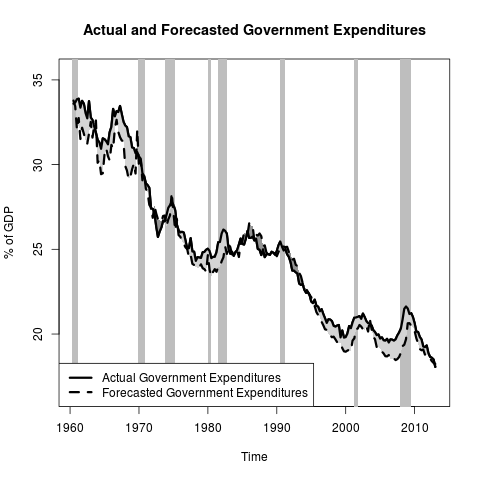
\includegraphics[scale=0.45]{./results/pics0.01/pred_gov.png} & 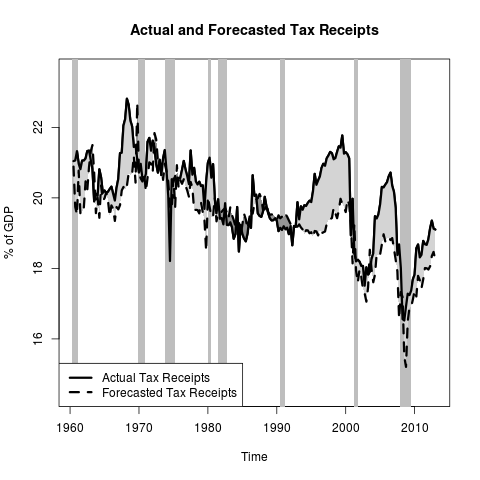
\includegraphics[scale=0.45]{./results/pics0.01/pred_tax.png} \\
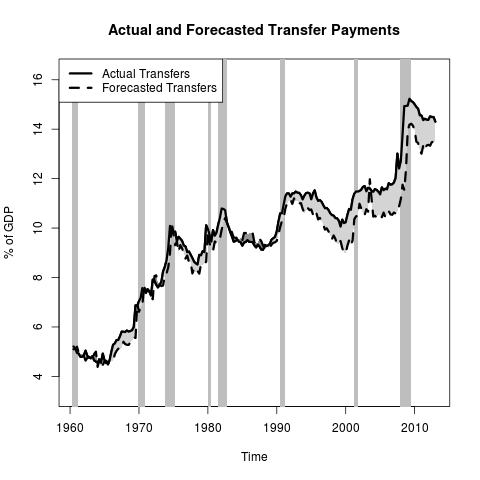
\includegraphics[scale=0.45]{./results/pics0.01/pred_transfers.png} & 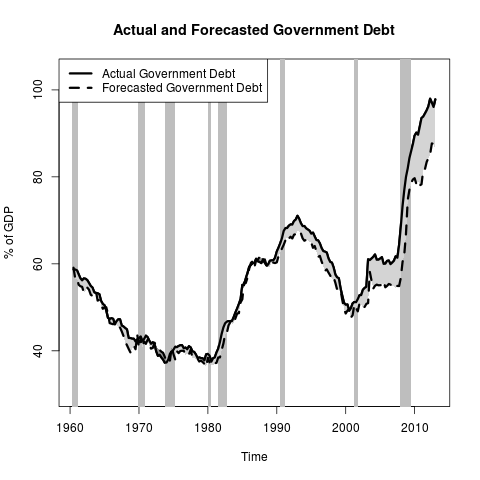
\includegraphics[scale=0.45]{./results/pics0.01/pred_debt.png}  
\end{tabular}
\end{center}
\end{figure} 

\begin{figure}\caption{Least-Squares Learning Prediction Errors}\label{fg:fe0.01}
\begin{center}
\begin{tabular}{cc}
\multicolumn{2}{c}{Learning Gain = 0.01} \\ [0.5pc]
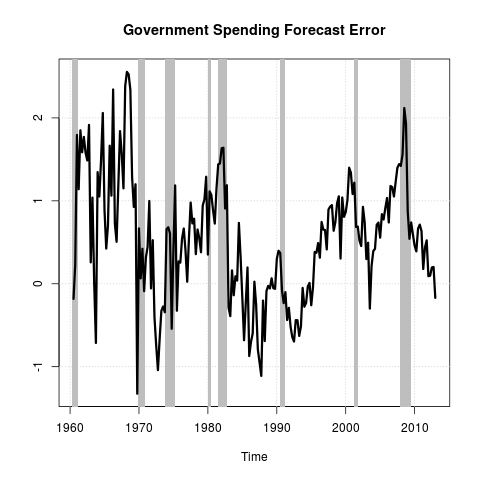
\includegraphics[scale=0.45]{./results/pics0.01/fe_gov.png} & 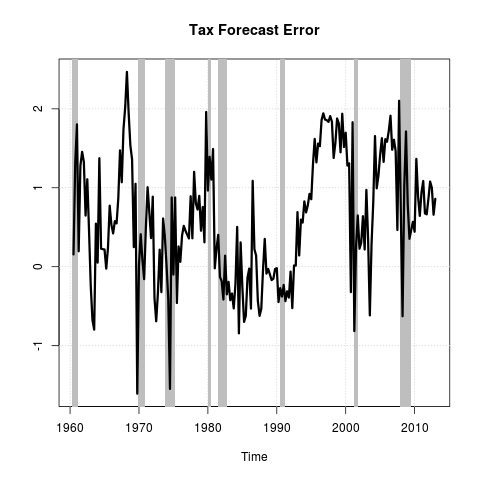
\includegraphics[scale=0.45]{./results/pics0.01/fe_tax.png} \\
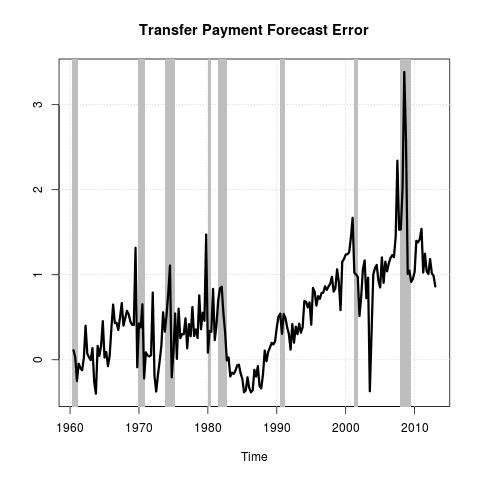
\includegraphics[scale=0.45]{./results/pics0.01/fe_transfers.png} & 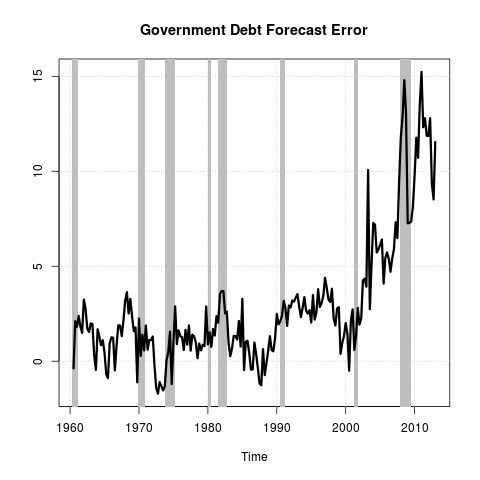
\includegraphics[scale=0.45]{./results/pics0.01/fe_debt.png}  
\end{tabular}
\end{center}
\end{figure} 

\begin{figure}\caption{Fiscal Policy Uncertainty}\label{fg:fpu0.01}
\begin{center}
\begin{tabular}{cc}
\multicolumn{2}{c}{Learning Gain = 0.01} \\ [0.5pc]
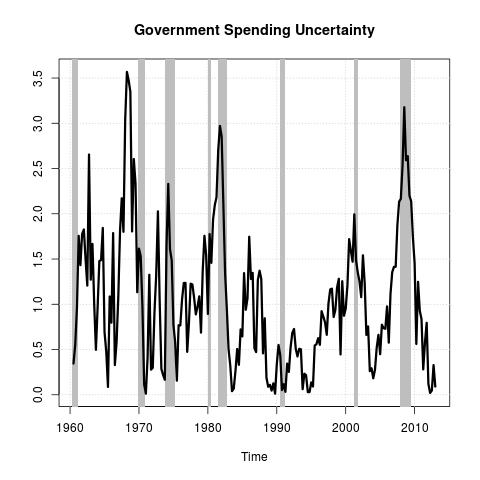
\includegraphics[scale=0.45]{./results/pics0.01/fpu_gov.png} & 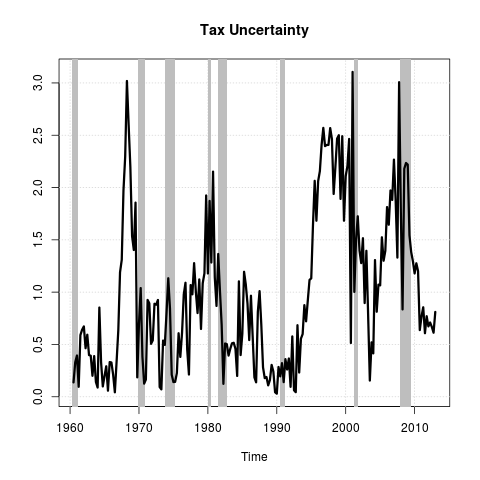
\includegraphics[scale=0.45]{./results/pics0.01/fpu_tax.png} \\
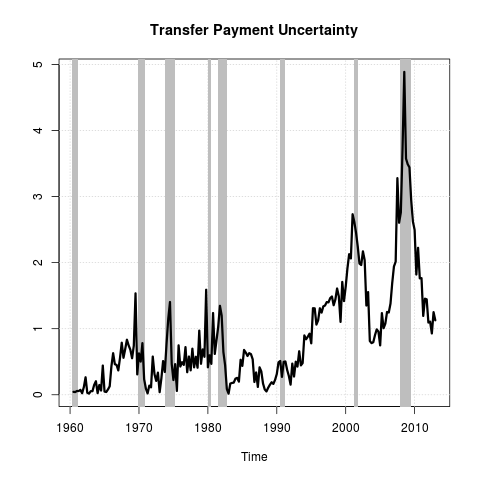
\includegraphics[scale=0.45]{./results/pics0.01/fpu_transfers.png} & 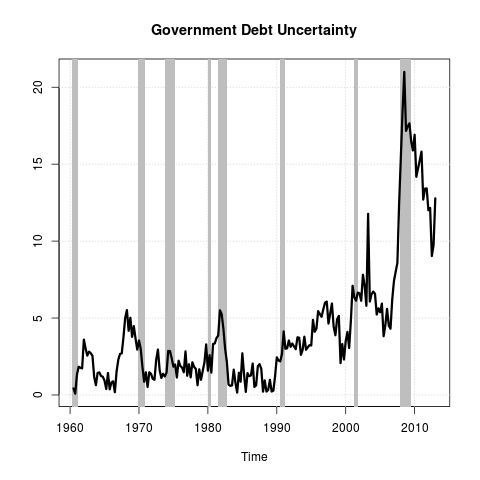
\includegraphics[scale=0.45]{./results/pics0.01/fpu_debt.png}  
\end{tabular}
\end{center}
\end{figure} 

\begin{figure}\caption{Least-Squares Learning Predictions}\label{fg:forecasts0.04}
\begin{center}
\begin{tabular}{cc}
\multicolumn{2}{c}{Learning Gain = 0.04} \\ [0.5pc]
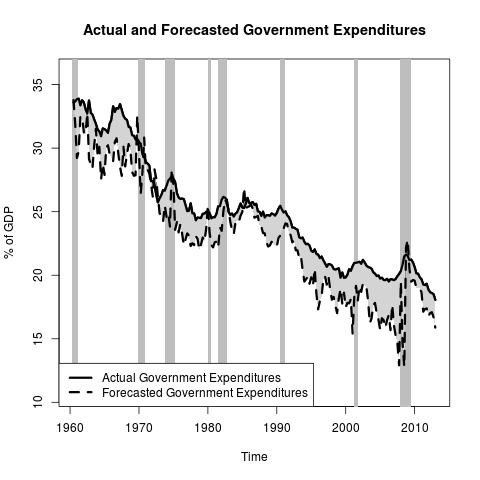
\includegraphics[scale=0.45]{./results/pics0.04/pred_gov.png} & 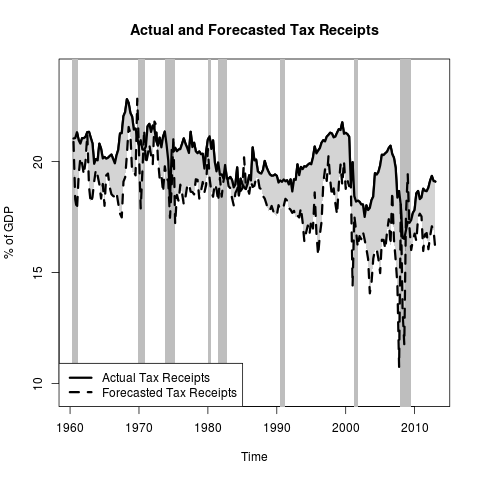
\includegraphics[scale=0.45]{./results/pics0.04/pred_tax.png} \\
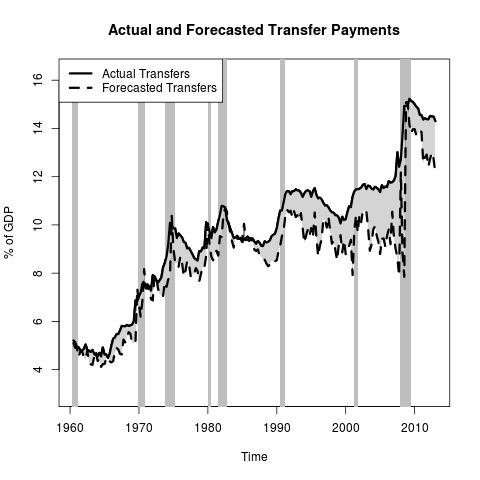
\includegraphics[scale=0.45]{./results/pics0.04/pred_transfers.png} & 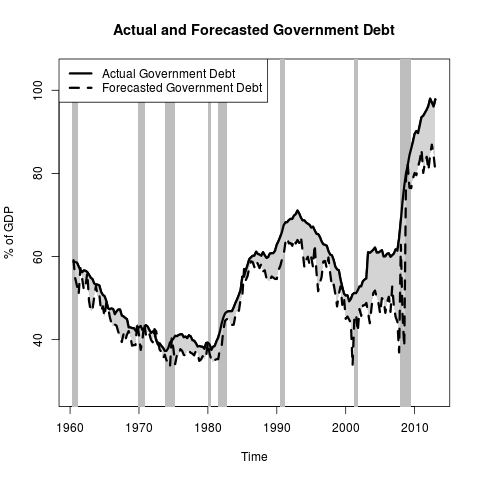
\includegraphics[scale=0.45]{./results/pics0.04/pred_debt.png}  
\end{tabular}
\end{center}
\end{figure} 

\begin{figure}\caption{Least-Squares Learning Prediction Errors}\label{fg:fe0.04}
\begin{center}
\begin{tabular}{cc}
\multicolumn{2}{c}{Learning Gain = 0.04} \\ [0.5pc]
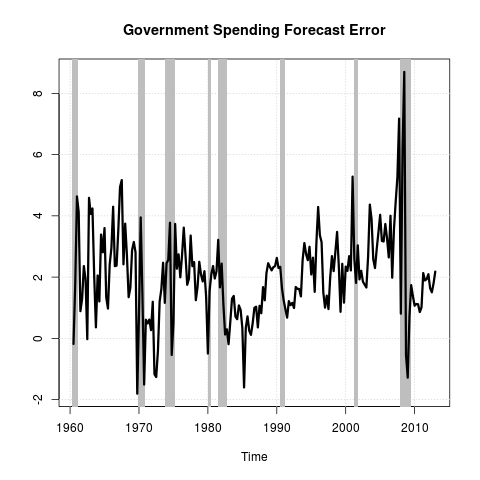
\includegraphics[scale=0.45]{./results/pics0.04/fe_gov.png} & 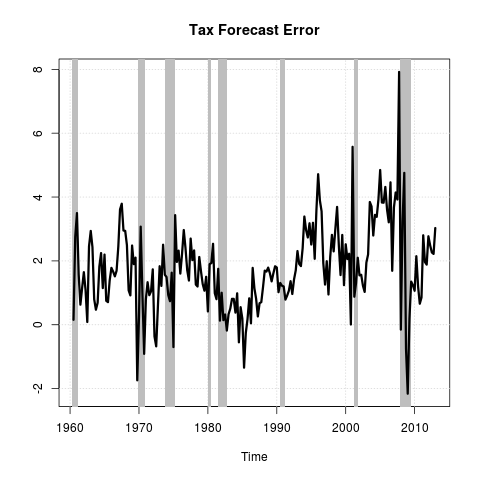
\includegraphics[scale=0.45]{./results/pics0.04/fe_tax.png} \\
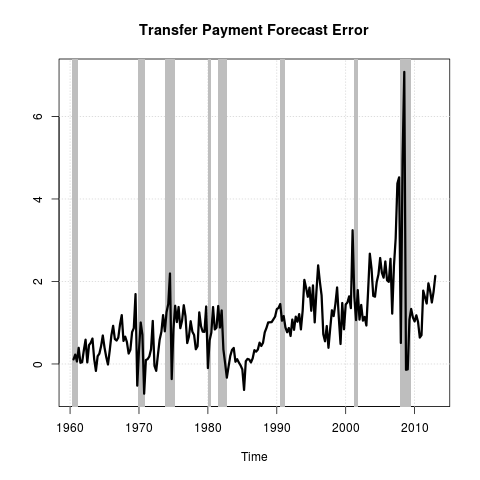
\includegraphics[scale=0.45]{./results/pics0.04/fe_transfers.png} & 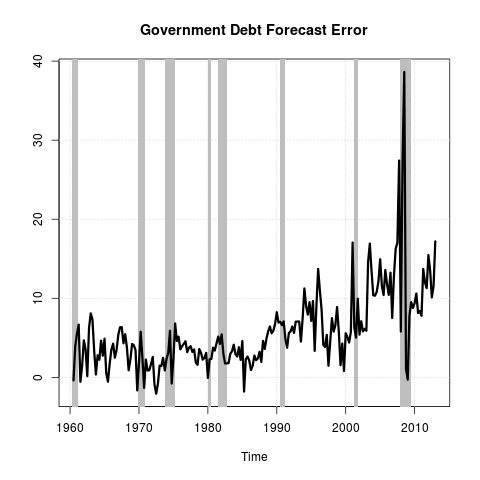
\includegraphics[scale=0.45]{./results/pics0.04/fe_debt.png}  
\end{tabular}
\end{center}
\end{figure} 

\begin{figure}\caption{Fiscal Policy Uncertainty}\label{fg:fpu0.04}
\begin{center}
\begin{tabular}{cc}
\multicolumn{2}{c}{Learning Gain = 0.04} \\ [0.5pc]
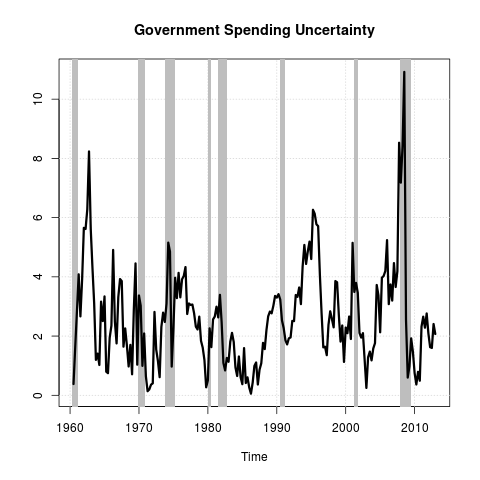
\includegraphics[scale=0.45]{./results/pics0.04/fpu_gov.png} & 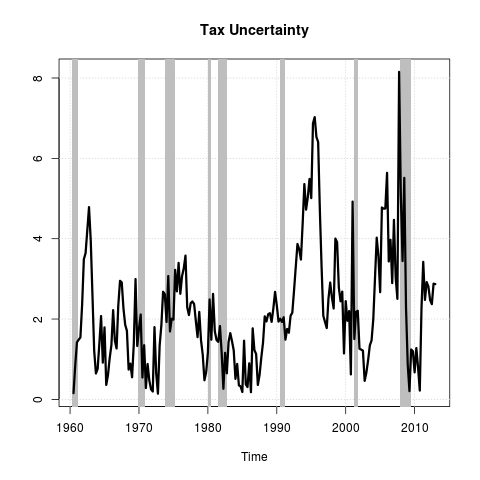
\includegraphics[scale=0.45]{./results/pics0.04/fpu_tax.png} \\
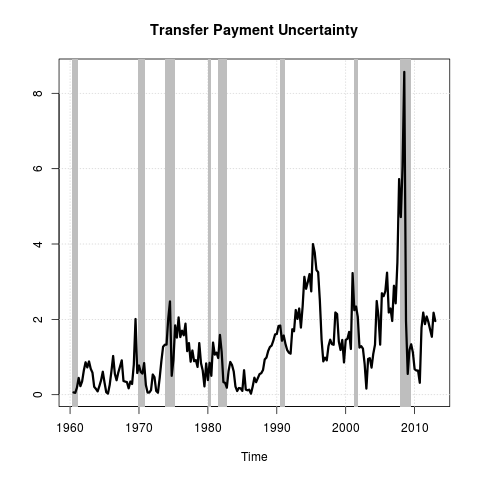
\includegraphics[scale=0.45]{./results/pics0.04/fpu_transfers.png} & 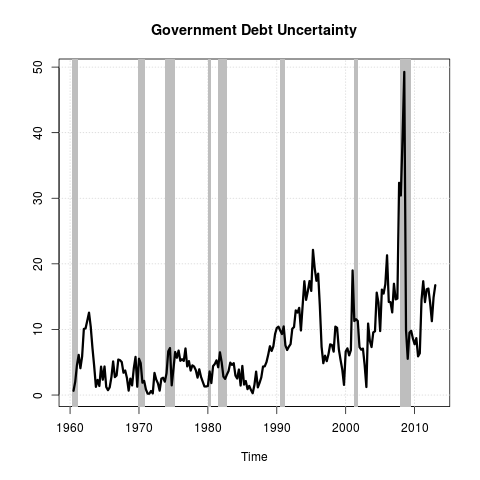
\includegraphics[scale=0.45]{./results/pics0.04/fpu_debt.png}  
\end{tabular}
\end{center}
\end{figure} 

\begin{figure}\caption{Unique Components of Fiscal Uncertainty}\label{fg:fpuremove0.01}
\begin{center}
\begin{tabular}{cc}
\multicolumn{2}{c}{Learning Gain = 0.01} \\ [0.5pc]
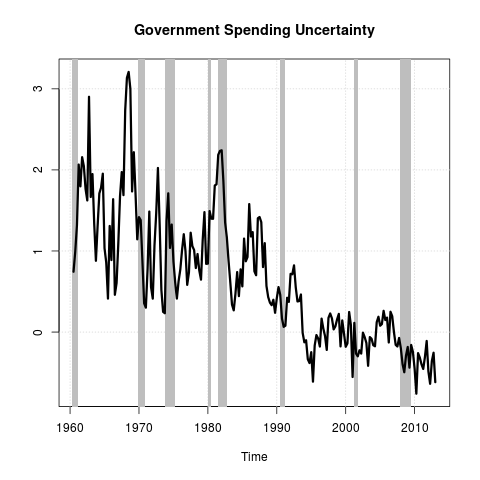
\includegraphics[scale=0.45]{./results/pics0.01/fpucoin_gov.png} & 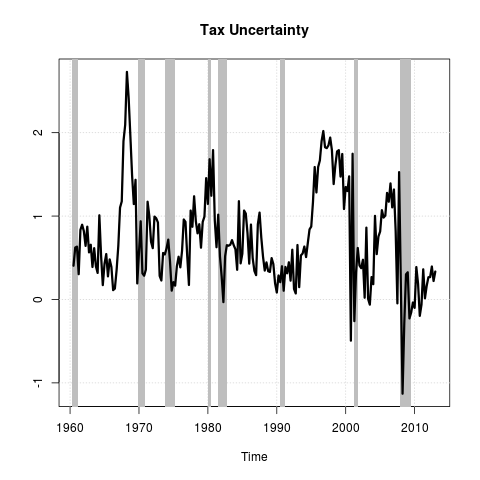
\includegraphics[scale=0.45]{./results/pics0.01/fpucoin_tax.png} \\
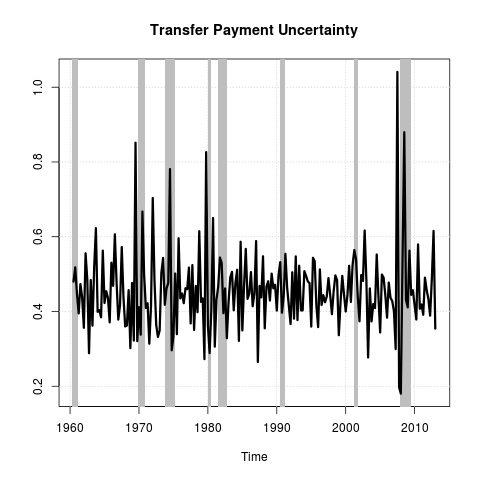
\includegraphics[scale=0.45]{./results/pics0.01/fpucoin_transfers.png} & 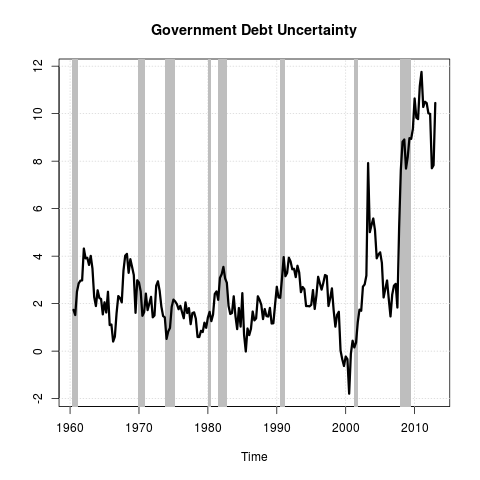
\includegraphics[scale=0.45]{./results/pics0.01/fpucoin_debt.png}  
\end{tabular}
\end{center}
\end{figure} 

\begin{figure}\caption{Unique Components of Fiscal Uncertainty}\label{fg:fpuremove0.04}
\begin{center}
\begin{tabular}{cc}
\multicolumn{2}{c}{Learning Gain = 0.04} \\ [0.5pc]
\includegraphics[scale=0.45]{./results/pics0.04/fpucoin_gov.png} & \includegraphics[scale=0.45]{./results/pics0.04/fpucoin_tax.png} \\
\includegraphics[scale=0.45]{./results/pics0.04/fpucoin_transfers.png} & \includegraphics[scale=0.45]{./results/pics0.04/fpucoin_debt.png}  
\end{tabular}
\end{center}
\end{figure} 

\end{document}
